\documentclass[russian,utf8,nocolumnsxix,nocolumnxxxi,nocolumnxxxii,nocolumnvii,nocolumnviii,floatsection,pointsubsection]{eskdtext}
\makeatletter
\newcommand{\updateStamp}{%
\savebox{\ESKD@stamp@ii@box}{%
\setlength{\unitlength}{1mm}%
\begin{picture}(0,0)(0,0)
\linethickness{\ESKDlineThick}
\put(0,40){\line(1,0){185}}
\put(0,30){\line(1,0){65}}
\put(0,25){\line(1,0){185}}
\put(135,20){\line(1,0){50}}
\put(135,15){\line(1,0){50}}
\linethickness{\ESKDlineThin}
\put(0,35){\line(1,0){65}}
\multiput(0,20)(0,-5){4}{\line(1,0){65}}
\linethickness{\ESKDlineThick}
\put(0,0){\line(0,1){40}}
\put(7,25){\line(0,1){15}}
\put(17,0){\line(0,1){40}}
\put(40,0){\line(0,1){40}}
\put(55,0){\line(0,1){40}}
\put(65,0){\line(0,1){40}}
\put(135,0){\line(0,1){25}}
\put(140,15){\line(0,1){5}}
\put(145,15){\line(0,1){5}}
\put(150,15){\line(0,1){10}}
\put(165,15){\line(0,1){10}}
\put(67, 1){\parbox[b][23mm][c]{66mm}{\centering\ESKDfontIII\ESKDtheColumnI}}
\put(67, 26){\parbox[b][13mm][c]{106mm}{\centering\ESKDfontVII\ESKDtheColumnII}}
\put(135, 21.3){\makebox[15mm]{\ESKDfontIII\ESKDcolumnIVname}}
\put(135, 16.3){\makebox[5mm][c]{\ESKDfontIII\ESKDtheColumnIVfI}}
\put(140, 16.3){\makebox[5mm][c]{\ESKDfontIII\ESKDtheColumnIVfII}}
\put(145, 16.3){\makebox[5mm][c]{\ESKDfontIII\ESKDtheColumnIVfIII}}
\put(150, 21.3){\makebox[15mm]{\ESKDfontIII%
  \ifESKD@twoside\ESKDcolumnVIItwosideName\else\ESKDcolumnVIIname\fi}}
\put(165, 21.3){\makebox[20mm]{\ESKDfontIII%
  \ifESKD@twoside\ESKDcolumnVIIItwosideName\else\ESKDcolumnVIIIname\fi}}
\put(137, 1){\parbox[b][13mm][c]{46mm}{\centering\ESKDfontV\ESKDtheColumnIX}}
\put(0.5, 21.3){\makebox[16mm][l]{\ESKDfontIII\ESKDcolumnXfIname}}
\put(0.5, 16.3){\makebox[16mm][l]{\ESKDfontIII\ESKDcolumnXfIIname}}
\put(0.5, 11.3){\makebox[16mm][l]{\ESKDfontIII\ESKDcolumnXfIVname}}
\put(0.5, 6.3){\makebox[16mm][l]{\ESKDfontIII\ESKDcolumnXfVname}}
\put(0.5, 1.3){\makebox[16mm][l]{\ESKDfontIII\ESKDcolumnXfVIname}}
\put(17.5, 21.3){\makebox[22mm][l]{\ESKDfontIII\ESKDtheColumnXIfI}}
\put(17.5, 16.3){\makebox[22mm][l]{\ESKDfontIII\ESKDtheColumnXIfII}}
\put(17.5, 11.3){\makebox[22mm][l]{\ESKDfontIII\ESKDtheColumnXIfIV}}
\put(17.5, 6.3){\makebox[22mm][l]{\ESKDfontIII\ESKDtheColumnXIfV}}
\put(17.5, 1.3){\makebox[22mm][l]{\ESKDfontIII\ESKDtheColumnXIfVI}}
\put(0, 26.3){\makebox[7mm]{\ESKDfontIII\ESKDcolumnXIVname}}
\put(7, 26.3){\makebox[10mm]{\ESKDfontIII\ESKDcolumnXVname}}
\put(17, 26.3){\makebox[23mm]{\ESKDfontIII\ESKDcolumnXVIname}}
\put(40, 26.3){\makebox[15mm]{\ESKDfontIII\ESKDcolumnXVIIname}}
\put(55, 26.3){\makebox[10mm]{\ESKDfontIII\ESKDcolumnXVIIIname}}
\end{picture}}}
\makeatother

% В рамке в поле с title уменьшить шрифт.
\renewcommand{\ESKDtheColumnI}{\ESKDfontIII\ESKDtheTitle\par\ESKDtheDocName\par\text{Пояснительная записка}}

\ESKDdepartment{Министерство образования РФ}
\ESKDcompany{Пензенский Государственный Университет}
\ESKDclassCode{31 1398}
\ESKDtitle{Распределенная агентно-ориентированная система доступа к базам данных}
\ESKDdocName{Технические условия}
\ESKDsignature{ПГУ 1.230101.24.001 ПЗ}
\ESKDauthor{Теренков~А.С.}
\ESKDtitleApprovedBy{%
a}{Гусев~И.~И.}
\ESKDtitleAgreedBy{%
a}{Иванов~И.~И.}
\ESKDtitleDesignedBy{%
a}{Теренков~А.С.}
\ESKDtitleDesignedBy{%
a}{Зинкин~С.А.}
\ESKDcolumnIX{ФВТ, каф. ВТ, гр 09ВВ1}
\ESKDchecker{Зинкин~С.А.}
\ESKDnormContr{Кучин~А.В.}
\ESKDsectSkip{subsection}{15mm}{10mm}
\ESKDsectSkip{subsubsection}{12mm}{8mm}
\ESKDdefaultFirstStyle{formIIab}
\usepackage{tocloft}
\usepackage{graphicx}
\usepackage{listings}
\usepackage{eskdtotal}
\usepackage{eskdlongtable}
\usepackage{multirow}
\usepackage{bigstrut}
\usepackage{textcase}
\usepackage{setspace}
\usepackage[T2A,T1]{fontenc}

\lstset{breaklines=true}
\lstset{basicstyle=\small\ttfamily}
\lstset{lineskip={-1.5pt}}
\captionsetup{font=small}
\graphicspath{{chapter0/}{chapter1/}{chapter2/}{chapter3/}}
\sloppy
\begin{document}
\makeatletter
\renewcommand{\paragraph}{\@startsection{paragraph}{4}{0ex}%
   {-3.25ex plus -1ex minus -0.2ex}%
   {1.5ex plus 0.2ex}%
   {\normalfont\normalsize\hspace{2mm}}}
\makeatother

\stepcounter{secnumdepth}
\stepcounter{tocdepth}

\renewcommand{\theenumi}{\arabic{enumi}}
\renewcommand{\cftsecleader}{\cftdotfill{\cftdotsep}}
\setcounter{secnumdepth}{4}

\ESKDdocName{Реферат}
\updateStamp
\ESKDthisStyle{formII}
\section*{Реферат}
\addcontentsline{toc}{section}{Реферат}
Пояснительная записка содержит \_\_ листов формата А4, \_ рисунков, \_ таблиц, 6 листов формата А1, 2 плаката формата А1, 10 источников, 4 приложения.

Распределенная агентно-ориентированная система доступа к базам данных.

РАСПРЕДЕЛЕННЫЕ ВЫЧИСЛИТЕЛЬНЫЕ СИСТЕМЫ, ПРОГРАММНЫЕ АГЕНТЫ, JADE, JAVA, БАЗЫ ДАННЫХ

Объектами исследования являются: распределенные системы, программные агенты, автоматизированный подход к сборке и развертыванию проектов.

Цель работы~--- разработка распределенной системы доступа к базам данных на основе технологии программных агентов.

В результате проведенной работы был реализован проект, удовлетворяющий поставленной задаче.

В пояснительной записке выполнено описание базовых понятий теории распределенных вычислительных систем, сделан обзор современных подходов к построению подобных решений,  представлено изложение принципов  автоматизированной сборки и развертывания приложений и рассмотрена работа с фреймворком Maven.

Графическая часть содержит модели UML.

\newpage
\section*{Список терминов и сокращений}
АОП~--- агентно-ориентированное программирование.

МАС~--- мультиагентная система.
 
ВС~--- вычислительная система.

СУБД~--- система управления базами данных.

ПЭВМ~--- персональная электронно-вычислительная машина.

UML (Unified Modeling Language)~--- унифицированный язык моделирования.

\maketitle
\newpage
\tableofcontents
\newpage
\ESKDdocName{Введение}
\updateStamp
\ESKDthisStyle{formII}
\section*{Введение}
\addcontentsline{toc}{section}{Введение}
Процессы мировой глобализации неразрывно связаны с развитием вычислительной техники и информационных технологий. Классические задачи, решаемые в рамках обособленного вычислительного узла, вытесняются задачами, требующими взаимной коммуникации и обмена ресурсами между инфомационными системами. В свою очередь это ведет к постоянному увеличению требований к имеющимся подходам и технологиям, предоставляющим подобные решения.

Одним из ведущих направлений в этой области является создание распределенных вычислительных систем, способных решать сложные и масштабные задачи путем взаимного сотрудничества и взаимодействия. Однако не любая совокупность объединеных компьютеров способна предоставить эффективный механизм решения крупных научных, производственных и технологических задач, поскольку, как показывают исследования, от подобных систем в процессе и принципах их функционирования требуется обеспечение следующего набора основных требований:

\begin{enumerate}
\item не требовать использования дополнительного дорогостоящего коммутационного оборудования;
\item быть достаточно простой в настройке и эксплуатации; не требовать для постоянного обслуживания высококлассных специалистов;
\item быть <<прозрачной>> для конечного пользователя, т.е. должна скрывать от него все тонкости ее функционирования;
\item быть <<самонастраиваемой>>, т.е. уметь поддерживать себя в активном состоянии в любых ситуациях (за исключением форсмажорных) без вмешательства человека;
\item поддерживать выполнение задач широкого класса;
\item быть надежно защищенной от вторжения извне.
\end{enumerate}

Вышеприведенный набор требований как нельзя лучше реализуется в рамках современной и перспективной концепции программных агентов, разработанных для решения сложных и масштабных проблем и задач. Одной из попыток показать это на реальном примере и является создение распределенной системы доступа к базам данных на основе агентно-ориентированного подхода в рамках данного курсового проекта. Перед этим будут описаны общие положения и теоретические основы данной предметной области, выполнено краткое описание современных подходов для решения подобных задач, их архитектурных особенностей, ключевых преимуществ и недостатков.

Также будет подробно описан агентно-ориентированный подход к программированию, показаны механизмы функционирования агентов, изучены их основные свойства и методы. Кроме того, будут рассмотрены принципы взаимодействия агентов между собой и их жизненные циклы.

Заключительным этапом проекта станет процесс непосредственной реализации работоспособной системы на основе программной среды разработки мультиагентных систем и приложений JADE, способной автономно функционировать в рамках поставленной задачи, предоставляя конечному пользователю унифицируемый доступ к имеющейся инфомации, расположенной на множестве компьютеров в сети.

Стоит отметить высокую актуальность рассматриваемой тематики, ее востребованность на современном рынке инфомационных технологий и программного обеспечения, а также недостаточную изученность и распространенность в широких кругах как в нашей стране, так за рубежом. Данный дипломный проект может послужить еще одним, пусть и небольшим вкладом среди пока еще узкого круга работ и материалов в области изучения, развития и реализации подхода построения распределенных вычислительных систем с использованием технологии программных агентов.

\section{Обзор предметной области и выбор инструментальной платформы}
\subsection{Распределенные вычислительные системы}
Парадигма распределенных вычислительных систем в настоящее время характеризуется стремительными темпами развития и эволюции используемых в ней идеологий и подходов. За непродолжительное время существования систем такого типа появилось множество различных схем организаций распределенных вычислений, набравших большой вес и общее признание, но практически исчезнувших впоследствии под давлением более новых и модных подходов. Такая ситуация зачастую ведет к тому, что исчезнувшая из виду технология появляется вновь под новым именем. В результате происходит непрерывное перемешивание базовых концепций с новейшими наработками. Для изучения и систематизации имеющихся технологий и подходов необходимо разобраться с базовыми понятиями и принципами организации систем подобного направления. 

\subsubsection{Понятие распределенной системы}
По утверждению известного специалиста в области информатики Э. Таненбаума, не существует общепринятого и в то же время строгого определения распределенной системы. 

Зачастую, при определении понятия <<распределенная система>> главное место отводят принципу разделения функционала между несколькими компьютерами. Однако при таком подходе распределенной является любая вычислительная система, в которой обработка данных разделена между двумя и более компьютерами. Сам Э.~Таненбаум в узком смысле определяет распределенную систему как набор соединенных каналами связи независимых компьютеров, которые с точки зрения пользователя некоторого программного обеспечения выглядят как единое целое.

\begin{figure}[h]
\center{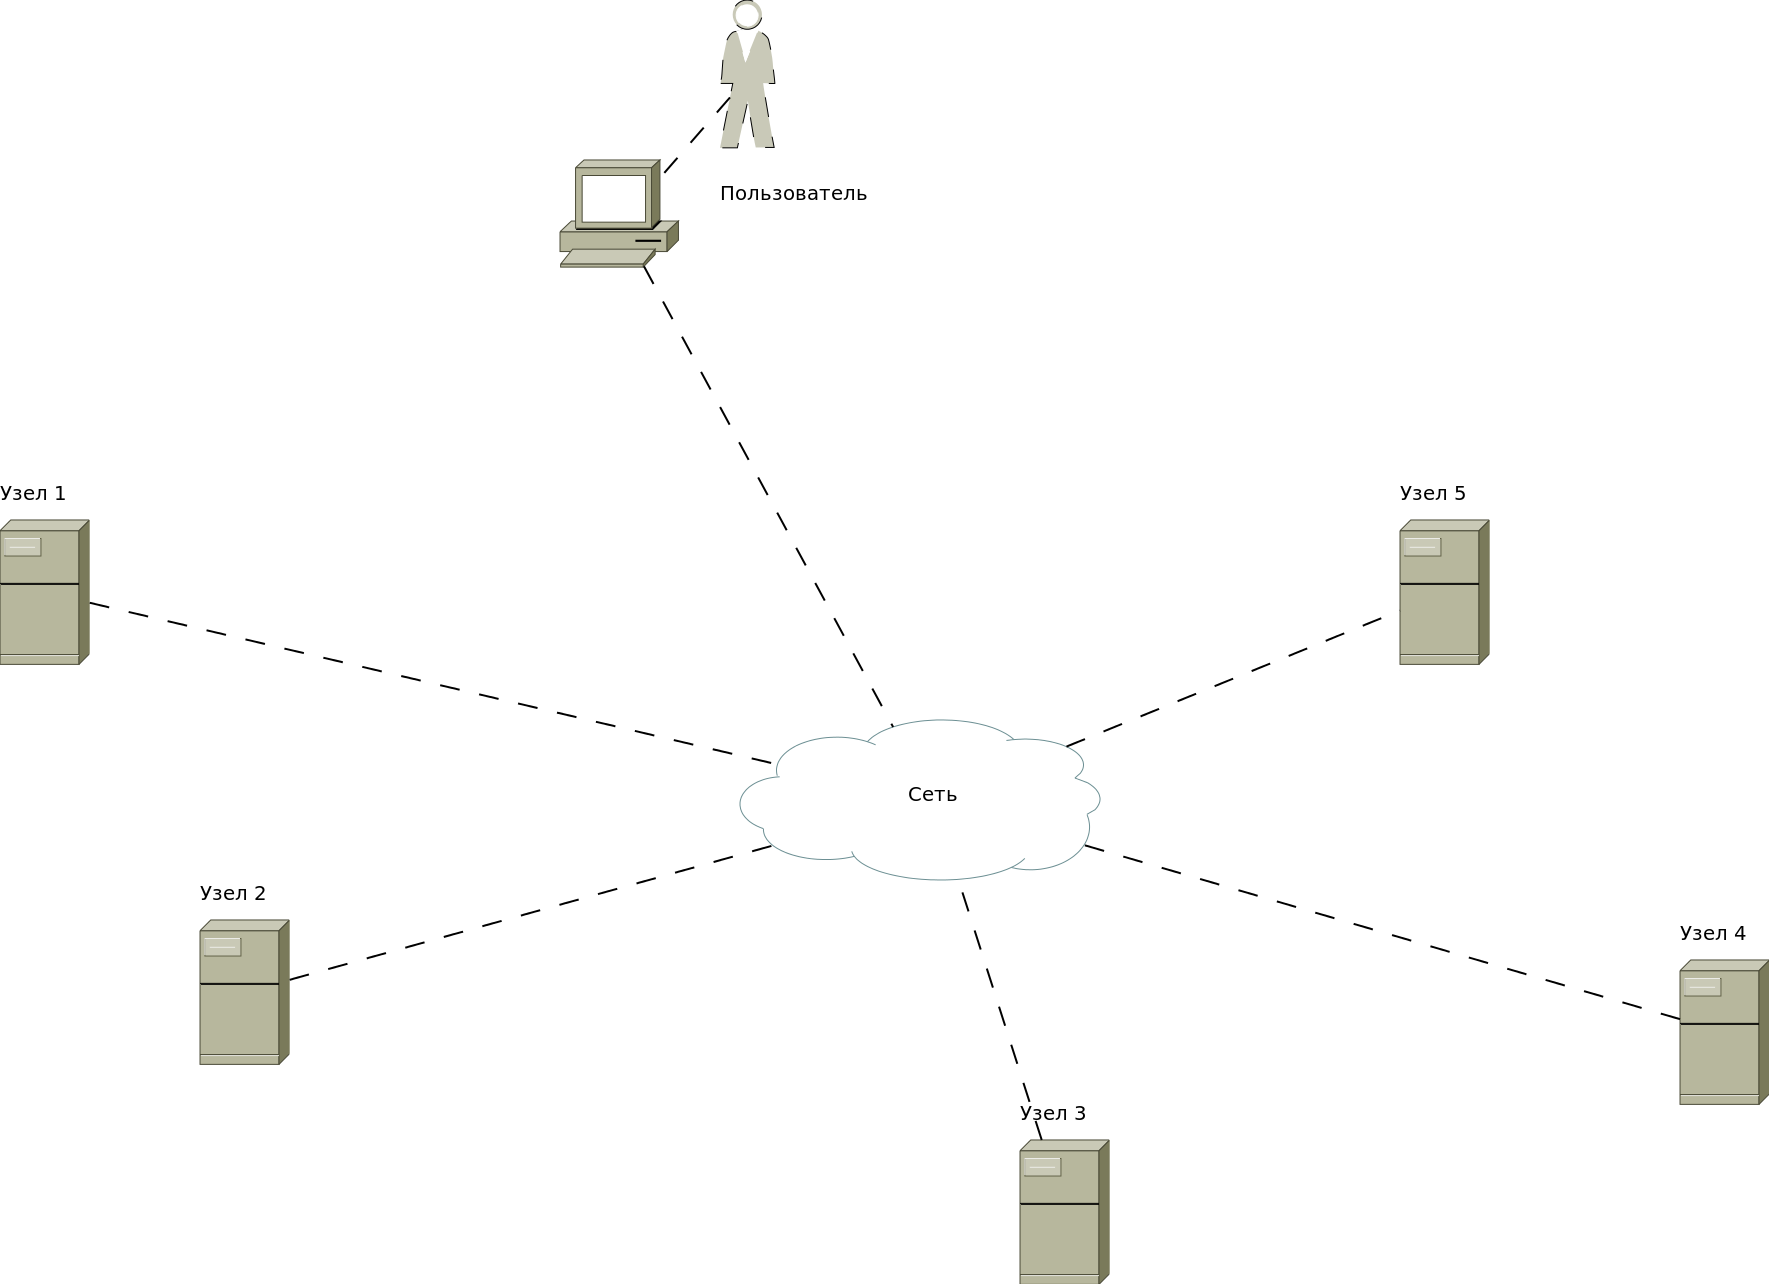
\includegraphics[width=1\linewidth]{dcs}}
\caption{Архитектура распределенной системы}
\label{0:dcs}
\end{figure}

В распределенных системах ключевым моментом является скрытие от пользователей различий между компьютерами и принципов организации их соединений (пользователь может даже не знать, что компьютер, используемый в системе, всего один). Пользователи и приложения единообразно работают в распределенных системах, независимо от того, где и когда происходит их взаимодействие. Вычислительная система, состоящая из множества различных вычислительных машин, на которых установлено различное программное обеспечение, может называться распределенной системой только в том случае, если для своих пользователей она выглядит и ведет себя как классическая однопроцессорная система с разделением времени. Чтобы поддерживать представление различных компьютеров и вычислительных сетей в виде единой системы, организация распределенных систем часто включает в себя дополнительный уровень программного обеспечения. Этот уровень называется уровнем системной поддержки.

Основная задача распределенных систем программного обеспечения~--- облегчить их пользователям доступ к удаленным ресурсам, а также организовывать их одновременное бесконфликтное использование. Зачастую, в классических системах совместное использование ресурсов достигается за счет тесного взаимодействия пользователей системы. Однако пользователь распределенной системы не должен знать, что он является не единственным ее пользователем. Ресурсы при этом могут быть как виртуальными, так и <<традиционными>>~--- компьютеры, принтеры, устройства хранения файлов и т.д.

\subsubsection{Основные понятия распределенных вычислительных систем}
\begin{enumerate}
\item Ресурс. Ресурсом называется любая программная или аппаратная сущность, представленная или используемая в распределенной сети. Например, компьютер, устройство хранения, файл, коммуникационный канал, сервис и т.п.
\item Узел~--- любое аппаратное устройство в распределенной вычислительной системе.
\item Сервер~--- это поставщик информации в распределенной вычислительной системе (например, веб-сервер).
\item Клиент~--- это потребитель информации в распределенной вычислительной системе (например, веб-браузер).
\item Пир~--- это узел, совмещающий в себе как клиентскую, так и серверную часть (т.е. поставщик и потребитель информации одновременно).
\item Сервис~--- это сетевая сущность, предоставляющая определенные функциональные возможности (например, веб-сервер может предоставлять сервис передачи данных по протоколу HTTP). В рамках одного узла могут предоставляться несколько различных сервисов.
\end{enumerate}

\subsubsection{Свойства распределенных систем}
\paragraph{Прозрачность системы}
Распределенная система должна скрывать разницу в способах представления данных и доступа к ресурсам. Такое свойство распределенных систем называется прозрачностью доступа к данным.

Прозрачность должна обеспечиваться и в отношении местоположения ресурса, то есть скрывать его физическое расположение. Важным условием функционирования системы является использование логических имен для ресурсов. Ресурс может время от времени менять свое расположение, и при следующем вызове может быть обнаружен в другом месте (но по тому же логическому адресу). Распределенная система, позволяющая ресурсам менять свое расположение от вызова к вызову, обладает свойством прозрачности смены местоположения ресурса. Иногда ресурс вынужден менять свое положение непосредственно в процессе его использования (пример такого ресурса~--- мобильные пользователи с беспроводной связью, не отключающиеся от сети при переходе в другую зону обслуживания). Это более сильное свойство называется прозрачностью динамической смены местоположения ресурса.

Для балансировки использования ресурсов может применяться операция реплицирования, т.е. <<размножения>> и распределения ресурсов по нескольким физическим адресам. Однако, это не должно оказывать влияния на способ взаимодействия пользователя с распределенной системой.

\paragraph{Открытость системы}

Открытость заключается в использовании синтаксических и семантических правил, основанных на стандартах. Для распределенной системы~--- это, прежде всего, заключается в использовании формализованных протоколов. Службы, входящие в распределенную систему, как правило, определяются через интерфейсы, которые часто описываются при помощи набора специальных языков (Interface Description Languages~--- IDL). При правильном описании интерфейса возникает возможность корректной совместной работы одного произвольного процесса, нуждающегося в интерфейсе, с другим произвольным процессом, представляющим этот интерфейс. Один и тот же интерфейс может быть также реализован в разных распределенных системах (независимо друг от друга), но работать обе системы должны одинаково.

Для обеспечения переносимости и способности к взаимодействию в интерфейсе должно быть все, что нужно для его реализации, но он не должен определять ее внешний вид. Переносимость характеризует, насколько приложение, сделанное для одной распределенной системы, может работать в составе другой системы, а способность к взаимодействию показывает, насколько две реализации систем или компонентов, выполненных разными людьми, в состоянии работать совместно. Открытые системы обладают очень важной характеристикой~--- гибкостью. Гибкость есть легкость конфигурирования системы, состоящей из различных компонентов. Достижения необходимого уровня гибкости приводит к тому, что открытая распределенная система становится расширяемой.

\paragraph{Масштабируемость системы}

Свойство масштабируемости также является неотъемлемой характеристикой распределенных вычислительных систем. Масштабируемость может проявляться по отношению к размеру, к географическому положению, к административному устройству систем. Достижение масштабируемости связано с решением проблем, возникающих из-за наличия узких мест по обслуживанию (один сервер для множества клиентов), данным (множественный доступ к одному файлу данных) и алгоритмам (перегрузка коммуникаций из-за использования централизованных алгоритмов). Требование масштабируемости зачастую является основным препятствием для распространения систем, реализованных для локальных сетей, на уровень корпоративных или глобальных, таких как интернет. В глобальных сетях, вследствие того, что узлы могут быть сильно удалены друг от друга в пространстве~--- время получения ответа может значительно превышать локальные задержки, поэтому там чаще используется асинхронная связь. Кроме того, в локальных сетях службы часто распределены по компьютерам фиксированно, а в глобальных~--- местоположение необходимой службы заранее неизвестно.

\subsubsection{Современные подходы к реализации распределенных вычислительных систем}
\paragraph{Peer-to-peer сети}
\begin{figure}[h]
\center{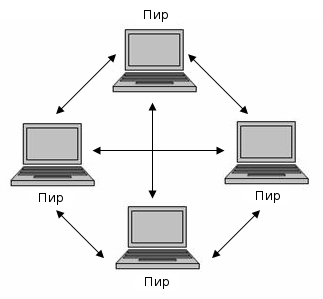
\includegraphics[width=0.6\linewidth]{peer}}
\caption{Организация peer-to-peer сети}
\label{0:peer}
\end{figure}

При работе в рамках парадигмы Peer-to-Peer (сокращенно P2P) компьютеры обмениваются ресурсами непосредственно друг с другом, без использования центрального сервера. Подход P2P обеспечивает решение проблем, возникших в результате экспоненциального роста интернет-сетей и веб-контента. Применение P2P позволило множеству польователей, которые раньше были простыми потребителями информации, поучаствовать в ее предоставлении. В момент своего появления P2P было скорее модным словом, чем продуманной концепцией. В результате мощного продвижения, в том числе, с помощью средств массовой информации, технология P2P распространилась в академических и промышленных кругах.

Основные достоинства одноранговых (Peer-to-peer) вычислительных систем:
\begin{itemize}
\item упрощается поддержка масштабируемости при значительном росте количества узлов в вычислительной сети; 
\item повышается отказоустойчивость сети, т.к. сбой любого вычислительного узла не может привести к остановке функционирования сети в целом.
\end{itemize}

Тем не менее, существует ряд препятствий при построении P2P сетей:
\begin{itemize}
\item при работе с P2P приложениями, вычислительный узел берет на себя функции как клиента, так и сервера. Это приводит к увеличению требований к производительности каждого компьютера, включенного в такую сеть.
\item низкая степень защищенности машин, участвующих в P2P сети объясняется тем, что они предоставляют открытый доступ к своим ресурсам (таким как такты процессора, определенные папки на жестком диске и т.п.). Таким образом, при отсутствии средств защиты, компьютеры, включенные в P2P подвержены риску взлома или заражения со стороны недобросовестных участников. 
\item при построении P2P сети приходится преодолевать возможную гетерогенность аппаратного и программного обеспечения ее потенциальных участников. Этот вопрос может быть решен путем применения таких технологий как XML, Java и т.д.
\item Основная проблема P2P сетей~--- это поиск доступных ресурсов без использования централизованной системы управления. Каждому узлу приходится производить поиск среди сотен и тысяч ресурсов внутри сети, что является весьма трудоемкой задачей.
\end{itemize}

\paragraph{Сервис-ориентированная архитектура}
В начале 2000-х годов мировое бизнес-сообщество занялось разработкой следующего поколения спецификаций, призванных решить проблемы ранних стандартов распределенных объектных технологий посредством веб-сервисов и сервис-ориентированной архитектуры (Service-Oriented Architecture~--- SOA).

\begin{figure}[h]
\center{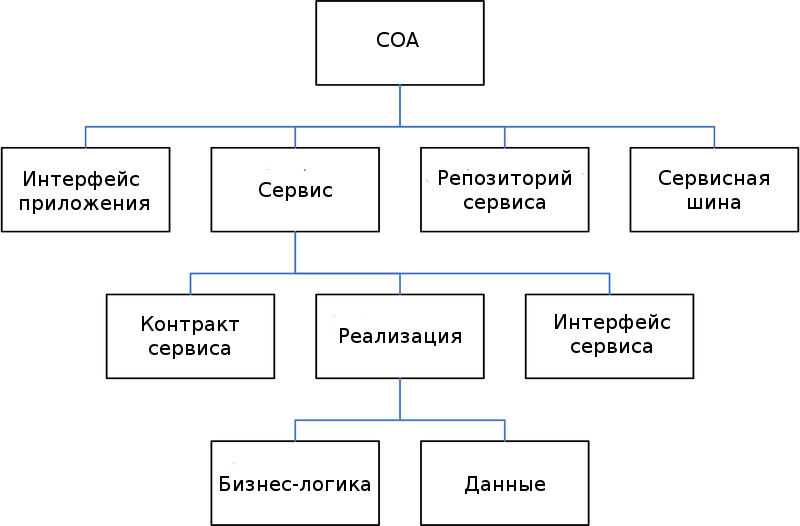
\includegraphics[width=1\linewidth]{soa}}
\caption{Одна из возможных реализаций архитектуры SOA}
\label{0:soa}
\end{figure}

Архитектура SOA не привязана к какой-либо определенной технологии. Она может быть реализована с использованием широкого спектра подходов: REST, RPC, DCOM, CORBA или веб-сервисов.

Главное, что отличает SOA~--- это использование независимых сервисов с четко определенными интерфейсами, которые для выполнения своих задач могут быть вызваны неким стандартным способом, при условии, что сервисы заранее ничего не знают о приложении, которое их вызовет, а приложение не знает, каким образом сервисы выполняют свою задачу.

SOA также может рассматриваться как стиль архитектуры информационных систем, который позволяет создавать приложения, построенные путем комбинации слабо-связанных и взаимодействующих сервисов. Эти сервисы взаимодействуют на основе какого-либо строго определенного платформо- и языко-независимого интерфейса (например, WSDL). Определение интерфейса позволяет скрывать внутреннюю реализацию сервиса.

Стандарты веб-сервисов были разработаны по инициативе организаций, занимающихся предоставлением удаленного доступа к определенным вычислительным ресурсам, и закреплены консорциумом W3C. К основным стандартам разработки и функционирования веб-сервисов можно отнести:
\begin{itemize}
\item SOAP~--- основанный на XML протокол взаимодействия веб-сервисов;
\item WSDL (Web Services Description Language~--- Язык описания веб-сервисов)~--- это методология описания ресурсов, предоставляемых веб-сервисом;
\item UDDI (Universal Description Discovery and Integration~--- Универсальный метод поиска и интеграции)~--- метод описания, поиска, взаимодействия и использования веб-сервисов. На сегодняшний день, сервис-ориентированный подход является стандартом «де-факто» при разработке распределенных вычислительных систем.
\end{itemize}

\paragraph{Программные агенты}
Несмотря на все преимущества технологии веб-сервисов, они не предоставляют новых методологий и решений построения широкомасштабных вычислительных сетей. Одним из вариантов решений, ведущихся в этом направлении, может быть рассмотрена агентно-ориентированная парадигма построения распределенных вычислительных систем. Вычислительные сети на основе так называемых программных агентов~--- это принципиально иной подход к организации систем и приложений.

Технология прогрммных агентов является основой реализации данного дипломного проекта, и будет детально рассмотрена в следующем подразделе.

\section{Описание и разработка распределенной системы доступа к базам данных на основе программных агентов платформы JADE}
\subsection{Краткое описание разрабатываемой системы}
Описываемая распределенная система разрабатывалась на объектно-ориентированном языке программирования Java. Ядром системы является программная платформа JADE, включающая в себя как набор классов для реализации агентно-ориентированных приложений, так и инструментарий для запуска, управления и настройки платформ, контейнеров и агентов.

	Для хранения данных используется свободная объектно-ориентированная система управления базами данных Postgresql. В качестве библиотеки с базой используется jdbc-драйвер. Взаимодействие системы с пользователем осуществляется с помощью стандартного графического оконного интерфейса на основе средств, представляемых библиотекой Swing.

	Управление процессом разработки осуществляется с помощью системы контроля версий GIT. Это позволяет контролировать все изменения в проекте, фиксировать контрольные точки и этапы разработки, а также мгновенно переключаться между ними. Исходный код проекта синхронизируется с сервером github.com. Это позволяет иметь доступ к проекту из любого места, где есть доступ к сети интернет.

	Сборка проекта, поиск и установка зависимостей осущестляется с помощью фреймворка Maven. Это позволяет в значительной мере сократить сроки и усилия по развертыванию, переносу, изменению конфигурации проекта и другим подобным операциям.

	Проектируемая распределенная система будет состоять из наборов взаимодействующих между собой программных агентов, часть из которых будет находиться на локальном контейнере платформы и обрабатывать пользовательские  запросы к базе, а часть~--- на удаленных контейнерах, имеющих в своем составе сервер базы данных, отвечая за обработку запросов от локальных агентов-клиентов, передачу этих запросов в СУБД, обработку и передачу ответа. Пользователь, взаимодействуя с графическим интерфейсом, будет формировать запросы, отправляемые первоначально на агент-контроллер, отвечающий за логику  межагентного взаимодействия, и получать ответы от удаленных серверов в главном окне программы.
\begin{figure}[h]
\center{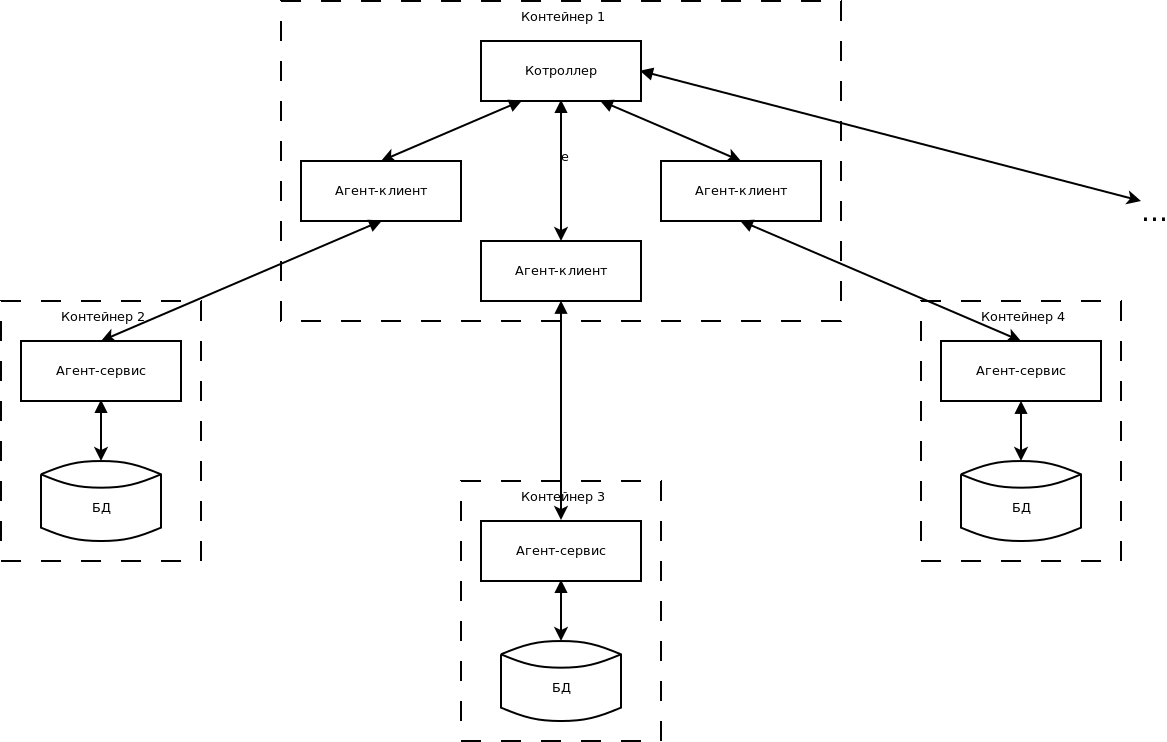
\includegraphics[width=0.9\linewidth]{common-scheme}}
\caption{Общая структура разрабатываемого приложения}
\label{3:common-scheme}
\end{figure}
Кроме этого, следует отметить, что изначально система запускается на локальном контейнере, а затем с помощью технологии мобильных агентов перемещает агенты-сервисы на имеющиеся в составе платформы удаленные контейнеры. Это позволяет иметь полную независимость от конфигураций серверных машин, версий и взаимной совместимости сервисной части системы на каждом удаленном узле. Более того, не потребуется помощь технического специалиста по настройке системы на каждом узле, не потребуется помощь и при масштабировании системы. Приложению достаточно увидеть новый контейнер в составе системы (ествественно, имеющей в своем составе необходимые для функционирования системы зависимости: JADE-платформа, без которой в общем-то и невозможно взаимное обнаружение и взаимодействие контейнеров внутри платформы, СУБД postgresql и т.д.), после чего, по указанию пользователя, будет произведена загрузка агента-сервиса на удаленный контейнер и его дальнейшее функционирование в рамках распределенной системы.

	Ниже приведена диаграмма последовательности запуска приложения и добавления нового узла (контейнера) в состав распределенной системы. Подобная последовательность событий и действий является аналогичной (начиная с события регистрации нового контейнера) при добавлении новых узлов в состав системы.
\begin{figure}[h]
\center{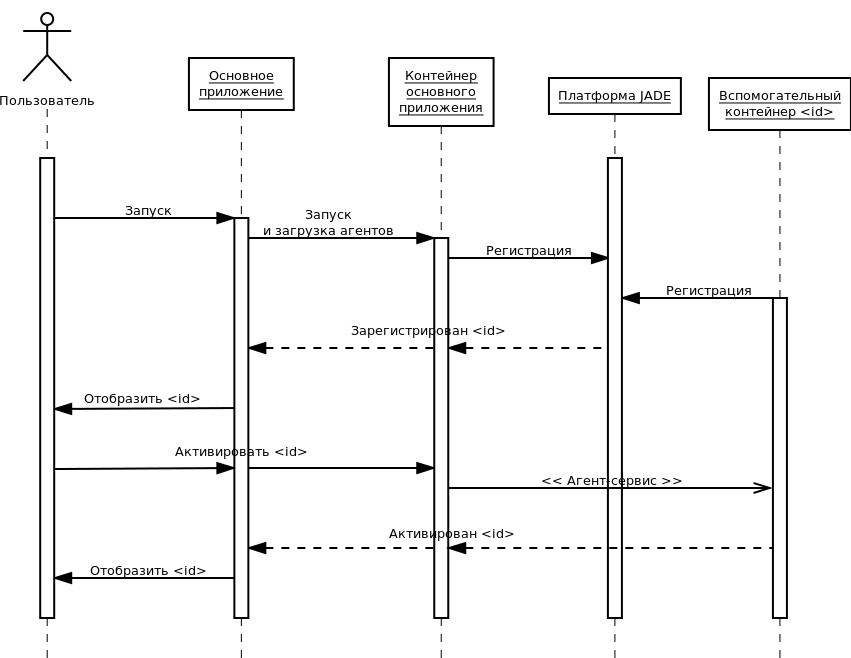
\includegraphics[width=0.9\linewidth]{seq-launch}}
\caption{Диаграмма последовательности запуска приложения и добавления нового узла}
\label{3:seq-launch}
\end{figure}
После загрузки агента-сервиса на удаленный контейнер происходит уведомление агента-контроллера, расположенного в составе модуля управления и  межагентного взаимодействия, после чего для агента-сервиса создается агент-клиент, который впоследствии будет уже напрямую обращаться к данному сервису.

Выбирая активные платформы, пользователь может обмениваться с ними информацией, не заботясь об их конфигурациях и местоположении.

Из доступных операций пользователю предоставляется возможность:
\begin{itemize}
\item получать список таблиц, расположенных на удаленном контейнере;
\item отображать контент выбранной таблицы контейнера;
\item редактировать данные выбранной таблицы;
\item добавлять данные в выбранную таблицу;
\item добавлять данные в выбранную таблицу с автоматическим реплицированием на активные контейнеры при наличии на них этой же таблицы;
\item выполнять RAWSQL-запросы на выбранный контейнер;
\item выполнять RAWSQL-запросы на все активные контейнеры.
\end{itemize}

\subsection{Описание состава пакетов системы}
\subsubsection{Состав пакета client}
Данный пакет содержит классы, входящие в состав агента-клиента. Основной класс ClientAgent, как видно из названия, реализует логику работы самого агента.

\paragraph{Класс ClientAgent}
Класс агента, как правило реализует основной метод setup(), в котором происходит инициализация агента, добавление поведений и другие операции, связанные с функционированием агента.
Ниже показано содержимое метода setup() класса ClientAgent:
\begin{verbatim}
protected void setup() {
    setEnabledO2ACommunication(true, 0);
    Object[] args = getArguments();

    switch(args.length) {
        case 3:
            serviceAID = (AID) args[2];
        case 2:
            agentInterface = (AgentInterface) args[1];
        case 1:
            ConditionalVariable startUpLatch = (ConditionalVariable) args[0];
            startUpLatch.signal();
    }

    ((AgentEvents) agentInterface).onEvent(new AID(getName(), AID.ISLOCALNAME), AgentEvents.EVENT_CLIENT_READY);
    addBehaviour(new O2ABehaviour());
}
\end{verbatim}
По-сути, содержимое метода отвечает за настройку приема данных от внешних классов, не являющихся агентами. Это реализовано с помощью технологии Object2Agent communication. Для этого необходимо включить поддержку взаимодействия O2A методом setEnabledO2ACommunication().

Далее, в контрукции switch() происходит выборка доступных аргументов, с которыми был запущен агент.

Первым аргументом (порядок аргументов идет с конца) передается мьютекс ConditionalVariable, который позволяет внешнему окружению дождаться запуска и инициализации агента. В противном случае, данные агентом получены не будут.

Второй аргумент хранит подписчика на события агента. Интерфейс AgentInterface имеет два интерфейса-потомка: AgentData и AgentEvents. Первый из них отвечает за уведомление о поступающих от агента данных, а второй~--- о возникающих событиях. В данном случае, агент посылает событие EVENT\_CLIENT\_READY, означающее готовность агента к функционированию.

Третий аргумент хранит AID~--- идентификатор~--- агента-сервиса, за которым <<закреплен>> данный агент-клиент.

В конце метода происходит добавление поведения O2ABehaviour, которое обрабатывает входящие данные от внешних модулей приложения.

\paragraph{Класс ClientBehaviour}
Основным методом объектов класса Behaviour является метод action(). Данный метод вызывается платформой по правилам, заложенным в реализации класса.

\begin{verbatim}
public void action() {
    ACLMessage message = null;

    switch (state) {
        case SENDING:
            message = new ACLMessage(ACLMessage.REQUEST);
            message.addReceiver(aid);

            try {
                message.setContentObject(agentDataContainer);
            } catch (IOException e) {
                e.printStackTrace();
            }

            myAgent.send(message);
            state++;
            break;
        case RECEIVING:
            message = myAgent.receive();
            if(message != null) {
                try {
                    agentDataContainer = (AgentDataContainer) message.getContentObject();
                } catch (UnreadableException e) {
                    e.printStackTrace();
                }

                AgentData agentData = (AgentData) ((ClientAgent) myAgent).getAgentInterface();
                AID aid = new AID(myAgent.getName(), AID.ISLOCALNAME);
                agentData.onData(aid, agentDataContainer);
                done = true;
            } else {
                block();
            }

            break;
    }
}
\end{verbatim}
Функционирование основного поведения агента-клиента реализовано в виде <<машины состояний>>. На первом этапе поведение функционирует в состоянии отправки запроса агенту сервиса, для чего формируется соотвестствующее ACL сообщение. На втором~--- в ожидании ответа от сервиса. В конце выполнения поведения происходит уведомление агента о полученных данных от агента-сервиса.

\paragraph{Класс O2ABehaviour}
Класс O2ABehaviour содержит циклический опрос очереди O2A-сообщений. При отсутствии сообщений поведение блокируется методом block() до появления нового сообщения в очереди.
\begin{verbatim}
public void action() {
    AgentDataContainer agentDataContainer = (AgentDataContainer) myAgent.getO2AObject();
    if(agentDataContainer != null) {
        myAgent.addBehaviour(new ClientBehaviour(myAgent, agentDataContainer));
    } else {
        block();
    }
}
\end{verbatim}

\subsubsection{Состав пакета service}
\paragraph{Класс ServiceAgent}
Основной класс пакета service~--- ServiceAgent. Его метод setup() аналогичен содержимому метода класса ClientAgent. Помимо этого, класс ServiceAgent реализует методы beforeMove() и afterMove()~--- это callback-методы, вызываемые платформой JADE, соотвественно до и после операции перемещения агента. Метод beforeMove() не содержит функциональной логики, а служит лишь для печати отладочной информации на консоль. Метод afterMove() добавляет новое поведение в состав агента, и посылает сообщение агенту-контроллеру о своем перемещении.
\begin{verbatim}
protected void afterMove() {
    addBehaviour(new ServiceBehaviour(this));

    System.out.println("After move: " + here());
    ACLMessage msg = new ACLMessage(ACLMessage.INFORM);
    msg.setConversationId(ControllerAgent.CONTROLLER_AGENT_CONVERSATION_ID);
    AID dest = new AID(ContainerHoldersManager.CONTROLLER_AGENT_NAME, AID.ISLOCALNAME);
    msg.setContent(getName());
    try {
        msg.setContentObject(here());
    } catch (IOException e) {
        e.printStackTrace();
    }
    msg.addReceiver(dest);
    send(msg);
}
\end{verbatim}
\paragraph{Класс ServiceAgent}
Поведение агента-сервиса ServiceBehaviour содержит интерфейсы взаимодействия с базой данных узла посредством классов, предоставляемых пакетом db. Логически поведение разбито на две части: это обработка запроса с передачей его к СУБД и формирование и отправка ответа агенту-клиенту. Кроме этого, при получении сообщения с типом CANCEL сервис завершает свою работу.
\begin{verbatim}
public void action() {
    ACLMessage msg = myAgent.receive();
    if (msg != null) {
        switch (msg.getPerformative()) {
            case ACLMessage.REQUEST:
                ACLMessage reply = msg.createReply();
                reply.setPerformative(ACLMessage.INFORM);
                AgentDataContainer agentDataContainer = null;

                try {
                    agentDataContainer = (AgentDataContainer) msg.getContentObject();
                    System.out.print(agentDataContainer);
                } catch (UnreadableException e) {
                    e.printStackTrace();
                }

                agentDataContainer = dbw.execute(agentDataContainer);
                agentDataContainer.setParam(AgentDataContainer.KEY_CONTAINER_NAME, myAgent.here().getName());

                try {
                    reply.setContentObject(agentDataContainer);
                } catch (IOException e) {
                    e.printStackTrace();
                }

                myAgent.send(reply);
                break;
            case ACLMessage.CANCEL:
                myAgent.doDelete();
                break;
        }
    } else {
        block();
    }
}
\end{verbatim}

\subsubsection{Состав пакета ctrl}
Пакет ctrl включает в себя классы, осуществляющие организацию межагентного взаимодействия, управление контейнерами, входящими в состав платформы, уведомление внешних внеагентных компонентов о событиях внутри платформы.
\paragraph{Класс ControllerAgent}
Запускает поведение мониторинка контейнеров платформы.

Уведомляет основной программный контроллер ContainerHolderManager о процедуре перемещения агентов-сервисов.

\paragraph{Класс AMSListenerBahaviour}
Данное поведение регистрирует обработчик в плтаформе JADE. Внутри обработчика добавления новых контейнеров просходит получение идентификатора контейнера и передача его контроллеру приложения.
\begin{verbatim}
public class AMSListenerBehaviour extends AMSSubscriber {
    public void installHandlers(Map handlersTable) {
        handlersTable.put(AddedContainer.NAME, new AddedContainerHandler());
    }

    public final class AddedContainerHandler implements EventHandler {
        public void handle(Event ev) {
            AddedContainer event = (AddedContainer) ev;
            ContainerID addedContainer = event.getContainer();

            ContainerHoldersManager.onContainerAdded(addedContainer);
        }
    }
}
\end{verbatim}

\paragraph{Класс ContainerHolder}
Данный класс хранит всю информацию, относящующся к конкретному контейнеру, а также предоставляет все интерфейсы для взаимодействия агентов клиента и сервиса внешним компонентам приложения. Основые поля класса:

\begin{itemize}
\item AgentController client~--- агент-клиент, относящийся к данному контейнеру;
\item AID serviceID~--- идентификатор сервиса, который расположен на данному конейнеру;
\item ContainerID containerID~--- идентификатор контейнера;
\item isActive~--- флаг активности контейнера~--- активный контейнер имеет в своем составе запущенные агенты сервиса и клиента, относящиеся к данному контейнеру.
\end{itemize}

\begin{itemize}
\item doActivate()~--- активирует данный контейнер;
\item doExecute()~--- отправляет запрос на сервис. В качестве параметра передается объект класса AgentDataContainer;
\item onData()~--- callback-функция получения информации от сервиса;
\item onEvent()~--- callback-функция получения событий от сервиса.
\end{itemize}

\paragraph{Класс ContainerHoldersManager}
Класс ContainerHoldersManager служит для организации системы распределенных узлов. В нем хранится список доступных на платфрме контейнеров, а также создает системный контейнер и запускает агента-контроллера. Помимо этого, он занимается обработкой событий, поступающих от объектов класса ContainerHolder и, в свою очередь, делегирует эти события собственным подписчикам (listeners).

\subsubsection{Пакет db}
Данный пакет состоит лишь из одного класса: DBWorker, который отвечает за всю логику взаимодействия с базами данных. Основным методом данного класса является метод execute(), который, как видно из названия выполняет запрос к базе и обрабатывает полученный ответ для выдачи результата запрашиваемому агенту-сервису.
\begin{verbatim}
public AgentDataContainer execute(AgentDataContainer agentDataContainer) {
    ...
    String dataType = AgentDataContainer.VALUE_DATA_TYPE_TABLES;

    connection = DriverManager.getConnection(url, user, password);

    if (agentDataContainer.getParam(KEY_REQUEST_STRING).equals(GET_TABLES_LIST)) {
        resultSet = connection.getMetaData().getTables(null, "public", "%", new String[]{"TABLE"});
    } else if (agentDataContainer.getDataLength() > 0) {
        boolean verified = verify(connection, agentDataContainer);
        if(verified) {
            dataType = AgentDataContainer.VALUE_DATA_TYPE_EMPTY;
            pst = connection.prepareStatement(agentDataContainer.getParam(KEY_REQUEST_STRING));

            Object[] dataRow = agentDataContainer.getData().get(0);
            for (int i = 0; i < agentDataContainer.getDataWidth(); i++) {
                pst.setObject(i + 1, dataRow[i], agentDataContainer.getMetadata()[i].getType());
            }

            pst.executeUpdate();
        }

        resultSet = null;
    } else {
        dataType = AgentDataContainer.VALUE_DATA_TYPE_CONTENT;
        pst = connection.prepareStatement(agentDataContainer.getParam(KEY_REQUEST_STRING));

        resultSet = pst.executeQuery();
    }

    outputAgentDataContainer = ResponseMaker.makeResponse(resultSet, agentDataContainer);
    outputAgentDataContainer.setParam(KEY_DATA_TYPE, dataType);
    ...
    return agentDataContainer;
}
\end{verbatim}
В ветвлении if происходит определение типа входящего запроса:
\begin{itemize}
\item получение списка таблиц;
\item операция модификации/добавления данных в таблице;
\item операция получения данных из таблицы / RAW-SQL запрос.
\end{itemize}
Кроме того, в этом методе происходит верификация корректности запроса при обращении к таблицам: это необходимо для операций репликации на всех активных узлах.

Соединение создается в строке connection = DriverManager.getConnection(). Класс DriverManager заведует драйверами, соединениями, а также трассировкой. В данном случае вызывается статический метод getConnection(). Этот метод просматривает список драйверов и, если находит подходящий к указанному URL, то создает и возвращает соединение. В противном случае выбрасывает исключение с текстом: "No suitable driver found". В качестве аргументов данный метод принимает URL к базе, имя и пароль пользователя.

Запрос для исполнения формирутеся с помощью метода prepareStatement() класса Connection. Запрос может состоять как из одной лишь текстовой строки, так и содержать объекты-параметры. Первая задается непостредственно в аргуенте метода, а последние~--- добавляться в запрос методов setObject(). Исполнение производится методом executeQuery(), либо executeUpdate() для выполнения операций вставки и модификаций в базе.

Ниже представлена архитектура JDBC, в рамках которой взаимодействует и базой данный, в том числе, и данное приложение, используя JDBC server.
\begin{figure}[h]
\center{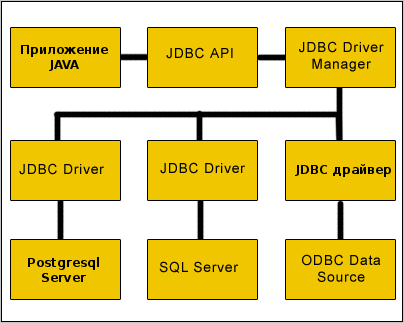
\includegraphics[width=0.7\linewidth]{jdbc}}
\caption{Взаимодействие Java-проложения с сервером БД}
\label{3:jdbc}
\end{figure}

\subsubsection{Пакет data}
\paragraph{Класс AgentDataContainer}
Данный класс является одним из наиболее универсальным и используемых сущностей в архитектуре приложения. Он пронизвыает буквально все уровни распределенной системы: начиная от классов графического пользовательского интерфейса, заканчивая обработчиком взаимодействия с сервером базы данных на удаленном узле. Данная унификация дает существенное преимущество: до тех пор, пока архитектурный уровень приложения не нуждается в содержимом информации, передаваемой другим уровням, он никак не вмешивается в их содержимое, структуру и методы, являясь лишь промежуточным звеном в коммуникационной цепочке. Это позволяет, при необходимости, изменять, дополнять, расширять архитектуру приложения, внося минимальные исправления в состав остальных компонентов.
\begin{figure}[h]
\center{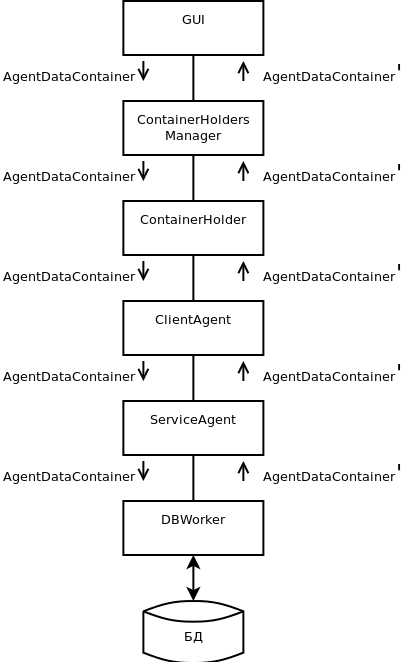
\includegraphics[width=0.5\linewidth]{comm-dia}}
\caption{Коммуникационная модель взаимодействия компонентов системы}
\label{3:comm-dia}
\end{figure}

Содержимое класса состоит из списка массива объектов, хранящих непосредственно табличные данные; массива типа <<Имя-Тип>> для хранения информации о типе и названии колонок данных; а также HashMap'a, содержащего набор <<Ключ-Значение>> для хранения таких параметров как: имя используемой таблицы, строки запроса и т.д.

\paragraph{Класс QueryMaker}
Класс QueryMaker реализует паттерн <<фабрика>> для объектов класса AgentDataContainer.

Основные методы класса:
\begin{itemize}
\item selectTables()~--- производит формирование запроса выборки списка таблиц базы;
\item selectTableContent()~--- производит выборку контента запрашиваемой таблицы;
\item insertData()~--- выполняет добавление строки данных в таблицу;
\item updateData()~--- выполняет модификацию строки данных в таблице.
\end{itemize}

\paragraph{Класс ResponseMaker}
Класс ResponseMaker выполняет сериализацию возвращаемого результа запроса к базе данных. Основной (и единственный) метод класса~--- makeResponse(). Результатом его работы является сформированный объект класса AgentDataContainer, хранящий данные, метадату и дополнительные параметры ответа: имя таблицы и хэш-код ее метадыты.
\begin{verbatim}
public static AgentDataContainer makeResponse(ResultSet resultSet, AgentDataContainer agentDataContainer) {
    NameTypePair[] metadata = null;
    List<Object[]> data = null;
    String metadataHash = "";

    if (resultSet != null) {
        try {
            ResultSetMetaData rsmd = resultSet.getMetaData();
            int columnCount = rsmd.getColumnCount();
            MetadataHasher.reset();

            metadata = new NameTypePair[columnCount];
            for (int columnIndex = 1; columnIndex <= columnCount; columnIndex++) {
                metadata[columnIndex - 1] = new NameTypePair();
                String name = rsmd.getColumnName(columnIndex);
                int type = rsmd.getColumnType(columnIndex);
                metadata[columnIndex - 1].setName(name);
                metadata[columnIndex - 1].setType(type);

                MetadataHasher.add(type, name);
            }
            metadataHash = MetadataHasher.get();

            data = new ArrayList<Object[]>();
            while (resultSet.next()) {
                Object[] row = new Object[columnCount];
                for (int columnIndex = 1; columnIndex <= columnCount; columnIndex++) {
                    row[columnIndex - 1] = resultSet.getObject(columnIndex);
                }
                data.add(row);
            }
        } catch (SQLException e) {
            e.printStackTrace();
        }
    }

    String tableName = agentDataContainer.getParam(KEY_TABLE_NAME);
    agentDataContainer = new AgentDataContainer(metadata,data);
    agentDataContainer.setParam(KEY_TABLE_NAME, tableName);
    agentDataContainer.setParam(KEY_METADATA_HASH, metadataHash);

    return agentDataContainer;
}
\end{verbatim}

\subsubsection{Пакет gui}
Набор классов данного пакета реализует графический пользовательский интерфейс приложения. Включает в себя следующие классы:
\begin{itemize}
\item ClientMainFrame~--- главное окно приложения;
\item ClientTable~--- табличный компонент для отображения данных;
\item ContainerHoldersList~--- список, отображающий доступные контейнеры платформы;
\item InsertDialog~--- модальное окно, осуществляющее добавление данных в таблицу.
\end{itemize}

\ESKDdocName{Технология автоматизированной сборки и развертывания проектов}
\updateStamp
\ESKDthisStyle{formII}
\section{Технология автоматизированной сборки и развертывания проектов с использованием фреймворка Maven}
\subsection{Концепция автоматизированной сборки программного обеспечения}
Непрерывные процессы усложнения программного обеспечения, сред и средств разработки, взаимной интеграции и использования составных частей различных технологий и приложений в одном проекте, использование методологий гибкой разработки ПО~--- зачастую делают традиционный подход к процессу ручной сборки программного обеспечения неоправнанно трудозатратным и малоэффективным.

Использование в процессе разработки систем управления версиями, таких как Git или CVS, на сегодняшний день является общепринятой практикой. Когда над одной системой работает большое число разработчиков, такая координация становится необходимой.  При этом важно быть уверенным, что последняя версия кода, находящаяся в системе управления версиями, всегда успешно собирается. Это хороший метод для проектов с замкнутыми командами разработчиков; когда разработчики периодически синхронизируют свои рабочие области с транком, несобирающийся исходный код задержит процесс разработки до исправления проблемы. Для проектов же с открытым исходным кодом сохранение основной ветки разработки в рабочем состоянии просто жизненно необходимо. Потенциальные программисты могут загрузить код в любой момент, и если он окажется в нерабочем состоянии~--- это с большой делей вероятности оттолкнет их от дальнейшего участия в таком проекте.

Другим современным аспектом разработки является подход, ориентированный на написание модульных тестов и включение их в выполнение на этапе сборки.
	Актуальная сегодня методология "экстремального программирования" (англ. Extreme Programming, XP) предполагает процесс непрерывной интеграции. Разработчики интегрируют свой код в основную ветку разработки как можно чаще~--- как правило, раз в несколько часов~--- проверяя при этом успешное выполнение всех тестов. Аналогичные методики итеративной разработки ПО придерживаются подобного подхода.

Для адаптации непрерывной интеграции и модульного тестирования необходимо, чтобы разработка проекта следовала этим методикам. Однако, зачастую этого недостаточно.

Итак, поскульку вышезложенные методы подходы состоят из неавтоматизированных шагов~--- интеграции кода, выполнения тестов и постоянном внесении кода в репозиторий~--- все это может повлечь технические трудности, излишние временные затраты и ошибки. Автоматизированная система, собирающая код и выполняющая модульные тесты, является гораздо более надежным решением.

\subsubsection{Требования к системам автоматизированной сборки ПО}
Базовые требования:
\begin{enumerate}
\item частые или <<ночные>> сборки для своевременного выявления проблем;
\item поддержка управления зависимостями исходного кода (Source Code Dependency Management);
\item обработка разностной сборки;
\item уведомление при совпадении исходного кода (после сборки) с имеющимися бинарными файлами;
\item ускорение сборки;
\item отчет о результатах компиляции и линковки.
\end{enumerate}

Дополнительные требования:
\begin{enumerate}
\item создание описания изменений (release notes) и другой сопутствующей документации (например, руководства);
\item отчет о статусе сборки;
\item отчет об успешном/неуспешном прохождении тестов;
\item суммирование добавленных/измененных/удаленных особенностей в каждой новой сборке.
\end{enumerate}

\subsubsection{Преимущества использования}
\begin{itemize}
\item улучшение качества продукта;
\item ускорение процесса компиляции и линковки;
\item избавление от излишних действий;
\item минимизация некорректных сборок;
\item избавление от привязки к конкретному человеку;
\item ведение истории сборок и релизов для разбора выпусков;
\item экономия времени и денег благодаря вышеобозначенных причинам,
\end{itemize}

\subsection{Система автоматизированной сборки Maven}
Apache Maven~--- фреймворк для автоматизации сборки проектов, специфицированных на XML-подобном языке POM (англ. Project Object Model). Maven обеспечивает декларативную сборку проекта. Это означает, что в файлах проекта pom.xml содержится его декларативное описание, а не отдельные команды. Все задачи по обработке файлов Maven выполняет через плагины.

\subsubsection{Преимущества Maven}
\begin{itemize}
\item независимость от OS. Сборка проекта происходит в любой операционной системе. При этом сборочный файл проекта остается неизменным от системы к системе;
\item управление зависимостями. Подавляющее большинство проектов пишутся с использованием сторонних библиотек (зависимостей). Эти сторонние библиотеки зачастую тоже используют другие библиотеки в качестве зависимостей. Maven позволяет управлять такими сложными процессами.  Это позволяет осуществлять поиск и установку нужного ПО, разрешать конфликты версий и, в случае необходимости, легко переходить на новые версии библиотек;
\item возможность сборки из командной строки. Такое часто необходимо для автоматической сборки проекта на сервере (практика использования подхода Continuous Integration);
\item хорошая интеграция со средами разработки. Основные среды разработки на Java без каких-либо сложностей поддерживают проекты, которые собираются c помощью фреймворка maven. При этом, зачастую, даже не требуется дополнительная настойка проекта~--- он сразу готов к дальнейшей разработке. Как следствие~--- если с проектом работают в разных средах разработки, то maven является отличным средством по унифицикации способа хранения настроек. Настроечный файл среды разработки и для сборки один и тот же~--- это уменьшает дублирование данных и, соответственно, количество ошибок;
\item декларативный стиль описания проекта. Позволяет лучшим образом формулировать конечные цели по организации проекта, не вдаваясь в детали и способы их реализации.
\end{itemize}

\subsubsection{Создание проекта под управлением maven}
Данные и последующие действия предполагают наличие установленного в системе фреймворка maven.

Для создания нового проекта необходимо ввети следующую команду:
\begin{lstlisting}
mvn archetype:generate
\end{lstlisting}
 
	Выполнив эту команду, maven покажет список шаблонов (архетипов) для разных проектов. Необходимо выбрать проект и его версию по умолчанию, Далее команда спросит groupId и artifactId.
В результате сгенерируется проект со стандартной структурой директорий:
\begin{lstlisting}
testproject1
|-- pom.xml
`-- src
    |-- main
    |   `-- java
    |       `--ru
    |           `-- ru.apache_maven
    |                   `-- App.java
    `-- test
        `-- java
            `-- ru
                `-- ru.apache_maven
                        `-- AppTest.java
\end{lstlisting}
        
В примере генерируется настройки приложения, включающего в себя помимо исходного кода набор JUnit-тестов и pom.xml~--- основной настроечный файл maven, который будет рассмотрен в следующем подразделе.

Чтобы скомпилировать код, нужно набрать в консоли: mvn compile. Успешная сборка проекта сопровождается следующим сообщением:

\begin{lstlisting}
.....
[INFO] BUILD SUCCESS
.....
\end{lstlisting}

Ввод команды “mvn package” в директории target сгенерирует jar файл testproject1-1.0-SNAPSHOT.jar.

\subsubsection{Основной файл проекта pom.xml}
pom.xml~--- это основной файл, описывающий проект. Вообще, в проекте могут использоваться дополнительные файлы, однако они играют второстепенную роль. Рассмотрим структуру файла pom.xml.

Корневой элемент и заголовок.

\begin{lstlisting}
<project xmlns="http://maven.apache.org/POM/4.0.0"
    xmlns:xsi="http://www.w3.org/2001/XMLSchema-instance"
    xsi:schemaLocation="http://maven.apache.org/POM/4.0.0
                    http://maven.apache.org/xsd/maven-4.0.0.xsd">
    <modelVersion>4.0.0</modelVersion>
    .............
</project>
\end{lstlisting}

Здесь находится корневой элемент <project>, схема, которая облегчает редактирование и проверку, и версия POM. Внутри тэга project содержится основная и обязательная информация о проекте:

\begin{lstlisting}
<!-- The Basics -->
  <groupId>...</groupId>
  <artifactId>...</artifactId>
  <version>...</version>
\end{lstlisting}

В Maven каждый проект идентифицируется парой groupId artifactId. Во избежание конфликта имен, в groupId заносится наименование организации или подразделения и обычно действуют такие же правила как и при именовании пакетов в Java~--- записывают доменное имя организации или сайта проекта. artifactId~--- название проекта. Внутри тэга version, как можно догадаться хранится версия проекта. Тройкой groupId, artifactId, version (далее~--- GAV) можно однозначно идентифицировать jar файл приложения или библиотеки. Если состояние кода для проекта не зафиксировано, то в конце к имени версии добавляется "\-SNAPSHOT"\,, что обозначает, что версия в разработке, и результирующий jar файл может меняться. <packaging>...</packaging> определяет какого типа файл будет создаваться как результат сборки. Возможные варианты pom, jar, war, ear.

Также добавляется информация, которая не используется самим мавеном, но нужна для программиста, чтобы понять, о чем этот проект:
\begin{itemize}
\item<name>powermock-core</name>~--- название проекта для человека;
\item<description>PowerMock core functionality.</description>~--- описание проекта;
\item<url>http://www.powermock.org</url>~--- сайт проекта.
\end{itemize}

\subsubsection{Зависимости}
Зависимости~--- следующая очень важная часть pom.xml~--- в данной секции хранится список всех библиотек (зависимостей) которые используюся в проекте. Каждая библиотека идентифицируется также как и сам проект~--- тройкой groupId, artifactId, version (GAV). Объявление зависимостей заключено в тэг <dependencies>...</dependencies>.

\begin{lstlisting}
<dependencies>
<dependency>
    <groupId>junit</groupId>
    <artifactId>junit</artifactId>
    <version>4.4</version>
    <scope>test</scope>
</dependency>
<dependency>
    <groupId>org.powermock</groupId>
    <artifactId>powermock-reflect</artifactId>
    <version>\${version}</version>
</dependency>
<dependency>
    <groupId>org.javassist</groupId>
    <artifactId>javassist</artifactId>
    <version>3.13.0-GA</version>
    <scope>compile</scope>
</dependency>
</dependencies>
\end{lstlisting}

Как можно заметить, кроме GAV при описании зависимости может присутствовать тэг <scope>. Scope задает спецификацию назначения данной библиотеки. В рассматриваемом примере указывается, что библиотека с GAV junit:junit:4.4 нужна только для выполнения тестов.

\subsubsection{Тэг <<build>>}
Тэг <build> является необязательным т.к. для него существуют значения по умолчанию. Этот раздел содержит информацию по самой сборке: где находятся исходные файлы, ресурсы проекта, список используемых плагинов.

\begin{lstlisting}
<build>
<outputDirectory>target2</outputDirectory>
<finalName>ROOT</finalName>
<sourceDirectory>src/java</sourceDirectory>
<resources>
    <resource>
        <directory>\${basedir}/src/java</directory>
        <includes>
        <include>**/*.properties</include>
        </includes>
    </resource>
</resources>
     <plugins>
         <plugin>
             <groupId>org.apache.maven.plugins</groupId>
             <artifactId>maven-pmd-plugin</artifactId>
             <version>2.4</version>
         </plugin>
     </plugins>
 </build>
\end{lstlisting}

Рассмотрим содержимое <build> секции.

\begin{itemize}
\item <sourceDirectory>~--- определяет, откуда maven будет брать файлы исходного кода. По умолчанию это src/main/java, но можно самостоятельно определить путь к исходному тексту. Директория может быть только одна (без использования специальных плагинов).
\item <resources> и вложенные в нее тэги <resource> определяют одну или несколько директорий, где хранятся файлы ресурсов. Ресурсы в отличии от файлов исходного кода при сборке просто копируются. Директория по умолчанию: src/main/resources 
\item <outputDirectory>~--- определяет, в какую директорию компилятор будут сохраняться результаты компиляции~--- *.class файлы. Значение по умолчанию: target/classes.
\item <finalName>~--- имя результирующего jar (war, ear..) файла с соответствующим типу расширением, который создается на фазе “package”. Значение по умолчанию: artifactId-version.
\end{itemize}

\subsubsection{Основные фазы сборки проекта}
\begin{itemize}
\item compile~--- компилирование проекта;
\item test~--- тестирование с помощью JUnit тестов;
\item package~--- создание .jar файла или war, ear в зависимости от типа проекта;
\item integration-test~--- запуск интеграционных тестов;
\item install~--- копирование .jar (war , ear) в локальный репозиторий;
\item deploy~--- публикация файла в удаленный репозиторий.
\end{itemize}

К примеру нам нужно создать jar проекта. Для его создания необходимо набрать:
\begin{lstlisting}
mvn package
\end{lstlisting}

Но перед тем как создаться jar файл будут выполняться все предыдущие фазы compile и test, а фазы integration-test, install, deploy не выполнятся. Если набрать:

\begin{lstlisting}
mvn deploy
\end{lstlisting}

то выполнятся все приведенные выше фазы.

Особым образом стоят фазы clean и site. Они не выполняются если специально не указаны в строке запуска.

\begin{itemize}
\item clean~--- удаление всех созданных в процессе сборки артефактов: .class, .jar и др. файлов. В простейшем случае результат~--- просто удаление каталога target;
\item site~--- предназначена для создания документации (javadoc + сайт описания проекта).
\end{itemize}

Т.к. команда mvn понимает когда ему передают несколько фаз, то для первоначальной сборки проекта и создания документации выполняют:

\begin{lstlisting}
mvn clean package site
\end{lstlisting}

\subsubsection{Будущее автоматизированных систем сборки проектов}
Вслед за появлением распределенных вычислительных систем обработки данных приходит время и нового поколения распределенных систем сборки проектов.  Термин <<распределенные сборки>> подразумевает, что вызовы компилятора и линковщика могут передаваться множеству компьютеров для ускорения скорости сборки.

Распределенный процесс сборки должен обладать определенной логикой, чтобы правильно определить зависимости в исходном коде для того чтобы выполнить этапы компиляции и линковки на разных машинах. Решение автоматизации сборки должно быть способно управлять этими зависимостями, чтобы выполнять распределенные сборки. Некоторые инструменты сборки могут распознавать подобные взаимосвязи автоматически (Rational ClearMake distributed, Electric Cloud ElectricAccelerator), а другие зависят от пользовательских указаний (Platform LSF lsmake) Автоматизация сборки, способная рассортировывать взаимосвязи зависимостей исходного кода, также может быть настроена на выполнение действий компиляции и линковки в режиме параллельного выполнения. Это означает, что компиляторы и линковщики могут быть вызваны в многопоточном режиме на машине, сконфигурированной с учетом наличия более одного процессорного ядра.

Далеко не все инструменты автоматизации сборки могут выполнять распределенные сборки. Большинство из них лишь реализует поддержку распределенной обработки (что далеко не то же самое). Кроме того, большинство решений, поддерживающих распределенные сборки, могут лишь обрабатывать код на языках Си и C++. Решения автоматизации сборки, поддерживающие распределенную обработку, зачастую основаны на Make и не поддерживают Maven или Ant.

В качестве примера решения распределенной сборки можно привести систему Xoreax’s IncrediBuild для платформы Microsoft Visual Studio. Это может потребовать специфической настройки программного окружения чтобы успешно функционировать на распределенной платформе (нужно указать расположение библиотек, переменные окружения и т. д.).

Из этого видно, что подход автоматизировнной сборки программного обеспечения является достаточно сложной и развитой технологией, позволяющей уже сегодня автоматизировать большую часть ручной работы по созданию целых систем и комплектов из наборов сложных стуртур изходных кодов, реусурсов, внешних зависимостей, библиотек и других компонентов проектов, обещая в ближайшем будущем сделать эти процессы еще более эффективными и технологичными, используя для этого уже описанные ранее преимущества концепции распределенных вычислений.

\section{Расчет затрат на разработку распределенной агентно-ориентированной системы доступа к базам данных}
\subsection*{Введение}
Целью данного дипломного проекта является разработка распределенной системы доступа к базам данных с использованием концепции программных агентов. Полученная разработка позволит иметь унифицированный доступ к инфомации, расположенной на множестве удаленных узлов.

В современном мире непрерывно происходят процессы глобализации и информационной интеграции. Они затронули и нашу страну, которая в силу географического положения и размеров вынуждена исользовать  распределенные информационные системы. Данные системы обеспечивают работу с данными, расположенными на разных серверах, различных аппаратно-программных платформах и хранящимися в различных форматах. Они легко расширяются, основаны на открытых стандартах и протоколах, обеспечивают интеграцию своих ресурсов с другими информационными системами, предоставляют пользователям простые интерфейсы. Это направление информационных технологий может успешно развиваться лишь при выполнении двух главных условий~--- адекватном развитии глобальной сетевой инфраструктуры и применении реальных технологий создания распределенных информационных систем. Второй аспект и является, по-преимуществу, объектом нашего исследования и рассмотрения.

Из этого следует, что актуальность затрагиваемой темы находится на высоком уровне. Действительно, наша страна прошла начальный этап глобальной компьютеризации. Многие решения по автоматизации малых и средних задач и проектов уже решаются адекватными средствами на достаточно высоком технологическом уровне. Но вот задачи совершенно иного качества – задачи создания глобальных распределенных информационных систем – нуждаются в осмыслении и анализе. Сложность настоящего этапа во многом предопределена традиционализмом и инерционностью мышления, выражающейся в попытке переноса средств и методов, применяемых для решения задач, обрабатываемых в рамках одного вычислительного узла, в мир глобальных систем, который живет по своим законам, требующим иных технологий.

Поведение и мотивация простых разработчиков вполне понятны и оправданы. Ставится задача~--- построить информационную систему <<клиент-сервер>> на базе локальной сети с централизованной базой данных. Для этого выбирается одна из популярных многопользовательских СУБД и какие-либо средства для быстрой разработки приложений (RAD). Далее создается сама система, которая являет собой комбинацию базы данных и обращающихся к ней приложений, в которых и реализована вся прикладная логика. И до тех пор, пока такая модель работает в ограниченном масштабе~--- все идет великолепно. Предположим, что организация, для которой выполнялась разработка, настолько выросла, что вновь возникшие задачи потребовали децентрализации хранения и обработки данных и, соответственно, развития информационной системы. Здесь и совершается ошибка. Подходы, хорошо зарекомендовавшие себя во вполне определенных условиях, автоматически переносятся в совершенно иную среду, с иными правилами жизнедеятельности. В результате система становится неработоспособной и должна быть создана заново, но уже с применением адекватных средств.

Децентрализованная система априори лишена подобных недостатков. Она отлично работает как в малых, так и средних и крупных масштабах ее использования: в первом случае отсутствуют техническая и экономическая избыточность, а во втором~--- система не приходит в непригодность и неработоспособность даже при глобальных изменениях архитектуры информационной топологии внутри организации.

Для реализации такой системы в данном проекте использовалась программная среда разработки мультиагентных систем и приложений JADE. В качестве инструмента разработки выступает объектно-ориентированный язык  программирования Java,~--- обладающий полной платформной независимостью, большим набором библиотечных функций и классов, обширной документацией и сообществом разработчиков, что несомненно оказывает положительное влияение на скорость и качество разработки, что в итоге оказывает влияние на конечную стоимость программного продукта. Разработка и функционирование разрабатываемой системы осуществляется на свободной операционной системе Linux.

\subsection{Расчет трудоемкости разработки}
Базовый показатель для определения составляющих затрат труда вычисляется по формуле:

\begin{center}
$ Q = q \cdot c (1 + p) $, где:
\end{center}

$q$~--- число операторов (исходных команд) в программном продукте;

$c$~--- коэффициент сложности программы; 

$p$~--- коэффициент коррекции программы в ходе ее разработки, зависит от точности и корректности поставленной задачи~--- принимаем равным 0,1.

Коэффициент сложности программы определяется из таблицы 1 на пересечении <<группы сложности>> и <<степени новизны>>. При этом новизна определяется по принципу:
\begin{itemize}
\item А~--- разработка  принципиально новых задач;
\item Б~--- разработка  оригинальных  программ;
\item B~--- разработка  программ  с использованием типовых решений;
\item Г~--- разовая  типовая  задача.
\end{itemize}

А сложность определяется исходя из типа решаемых задач:
\begin{itemize}
\item 1~--- алгоритмы  оптимизации и моделирования  систем;
\item 2~--- задачи  учета,  отчетности  и  статистики;
\item 3~--- стандартные  алгоритмы.
\end{itemize}

Кроме того, в таблице указан коэффициент недостаточности описания программы, который потребуется в дальнейшем.

\begin{center}
\begin{longtable}{|p{3cm}|p{3cm}|p{1.5cm}|p{1.5cm}|p{1.5cm}|p{1.5cm}|p{3cm}|}
\caption{Коэффициенты расчета трудоемкости}
\label{econom:trud}\\
\hline
\multirow{2}[4]{3cm}{\textbf{Язык }} &
\multirow{2}{3cm}{\textbf{Группа сложности}} &
\multicolumn{4}{c|}{\textbf{Степень новизны}} &
\multirow{2}{3cm}{\textbf{Коэффициент B}} \\
\cline{3-6}
 & & \textbf{А} & \textbf{Б} & \textbf{В} & \textbf{Г} &  \\
\hline
\endfirsthead
\caption*{Продолжение таблицы \thetable}\\
\hline
\multirow{2}[4]{3cm}{\textbf{Язык }} &
\multirow{2}{3cm}{\textbf{Группа сложности}} &
\multicolumn{4}{c|}{\textbf{Степень новизны}} &
\multirow{2}{3cm}{\textbf{Коэффициент B}} \\
\cline{3-6}
 & & \textbf{А} & \textbf{Б} & \textbf{В} & \textbf{Г} &  \\
\hline
\endhead
\endfoot
\hline
\endlastfoot
\multirow{3}{3cm}{Высокого уровня}
  & 1 & 1,38 & 1,26 & 1,15 & 0,69 & 1,2 \\
\cline{2-7}
  & 2 & 1,30 & 1,19 & 1,08 & 0,65 & 1,35 \\
\cline{2-7}
  & 3 & 1,20 & 1,10 & 1,00 & 0,60 & 1,5 \\ \hline

\multirow{3}{3cm}{Низкого уровня} 
  & 1 & 1,58 & 1,45 & 1,32 & 0,79 & 1,2 \\
\cline{2-7}
  & 2 & 1,49 & 1,37 & 1,24 & 0,74 & 1,35 \\
\cline{2-7}
  & 3 & 1,38 & 1,26 & 1,15 & 0,69 & 1,5 \\ \hline
\end{longtable}
\end{center}

Реализованная в дипломном проекте распределенная агентная система написана на языке высокого уровня Java, степень ее новизны обозначим коэффициентом <<Б>>, а группу сложности примем за единицу.

Таким образом, коэффициент сложности равен 1,26.

Общее число операторов в программе составляет 1287.

Базовый показатель $Q = 1,26 \cdot 1287 (1 + 0,1) = 1783,8$.

Далее, рассчитаем составляющие затраты труда, среди которых выделяют:

\begin{itemize}
\item затраты труда на подготовку и описание алгоритмов;
\item затраты труда на исследование алгоритмов;
\item затраты труда на разработку алгоритмов;
\item затраты труда на программирование и отладку.
\end{itemize}

Затраты труда на подготовку и описание задачи может определяться эмпирически или по формуле:

\begin{center}
$ t_\text{оп} = \frac{T_{min} + 4 \cdot T_\text{нв} + T_max}{6} = \frac{30 + 4 \cdot 60 + 90}{6} = 60$ (чел. час.), где:
\end{center}

$T_{max}$~--- трудоемкость операции в наиболее неблагоприятных условиях (пессимистическая оценка);

$T_{min}$~--- трудоемкость операции при благоприятных условиях (оптимистическая оценка); 

$T_\text{нв}$~--- трудоемкость операции при нормальных  условиях (наиболее вероятная оценка).

Ориентировочные величины оценки трудоемкости операции подготовки описания задачи в зависимости от числа операторов q приводятся в таблице~\ref{econom:desc}.

\begin{center}
\begin{longtable}{|p{4cm}|p{4cm}|p{4cm}|p{4cm}|}
\caption{Оценка времени подготовки описания задачи}
\label{econom:desc}\\
\hline
\textbf{q} & \textbf{$T_{min}$} & \textbf{$T_\text{нв}$} & \textbf{$T_{max}$} \\
\hline
\endfirsthead
\caption*{Продолжение таблицы \thetable}\\
\hline
\textbf{q} & \textbf{$T_{min}$} & \textbf{$T_\text{нв}$} & \textbf{$T_{max}$} \\
\hline
\endhead
\endfoot
\hline
\endlastfoot
             100 & 10 & 15 & 20 \\ \hline
             500 & 20 & 35 & 50 \\ \hline
            1000 & 25 & 50 & 75 \\ \hline
            1500 & 30 & 60 & 90 \\ \hline
            2000 & 40 & 70 & 100 \\ \hline
            2500 & 50 & 80 & 110 \\ \hline
            5000 & 70 & 110 & 150 \\ \hline
           10000 & 100 & 150 & 200 \\ \hline
\end{longtable}
\end{center}

Затраты труда на исследование алгоритма решения задачи определяются формулой:
\begin{center}
$ t_\text{ис} = \frac{Q \cdot B}{85 \cdot k}$ (чел. час.), где:
\end{center}

$Q$~--- базовый коэффициент;

$B$~--- коэффициент недостаточности описания задачи, который берется из таблицы~\ref{econom:desc}, в данном случае равен 1,2;

$k$~--- коэффициент квалификации программиста, зависит от стажа работника и определяется из таблицы~\ref{econom:skill} (принимается равным 1).

\begin{center}
    \begin{longtable}{|p{7cm}|p{10cm}|}
\caption{Коэффициенты квалификации программисты}
\label{econom:skill}\\
\hline
\textbf{Опыт работы} & \textbf{Коэффициент квалификации} \\
\hline
\endfirsthead
\caption*{Продолжение таблицы \thetable}\\
\hline
\textbf{Опыт работы} & \textbf{Коэффициент квалификации} \\
\hline
\endhead
\endfoot
\hline
\endlastfoot
             До двух лет & 0.8 \\ \hline
             2-3 года & 1 \\ \hline
             3-5 лет & 1.1-1.2 \\ \hline
             5-7 лет & 1.3-1.4 \\ \hline
             более 7 лет & 1.5-1.6 \\ \hline
\end{longtable}
\end{center}

Таким образом, время на исследование алгоритмов составляет:
\begin{center}
$ t_\text{ис} = \frac{1783,8 \cdot 1,2}{85} = 31$ (чел. час.)
\end{center}

Затраты труда на разработку архитектуры и схем алгоритмов составляют:

\begin{center}
$ t_\text{ал} = \frac{Q}{25 \cdot k} = \frac{1783,8}{25} = 71.4 $
\end{center}

Затраты труда на программирование системы по составленным алгоритмам и ее отладку:

разработка: $ t_\text{пр} = \frac{Q}{25 \cdot k} = \frac{1783,8}{25} = 71,4 $ (чел. час.)

отладка: $ t_\text{отл} = \frac{1783,8}{5} = 356,8 $ (чел. час.)

Суммарные затраты труда рассчитываются как сумма составных затрат труда:
$ t_\Sigma = t_\text{ис} + t_\text{ал} + t_\text{пр} + t_\text{отл} = 60 + 31 + 71,4 + 71,4 + 356,8 = 590,6 $ (чел. час.)

\subsection{Экономические расчеты}
\subsubsection{Расчет затрат на оборудование, амортизацию и обслуживание}
Для проведения работ по написанию и тестированию программы, с учетом специфики распределенных систем, использовались 3 компьютера и 1 роутер. Одна из машин использовалась как для непосредственного запуска и функционирования системы, так и для ее разработки, ввиду чего ее технические параметры должны существенно превышать параметры остальных <<пользовательских>> конфигураций системных блоков, используемых исключительно для запуска на них и отладки системы. Следовательно, и стоимость системного блока, используемого для разработки будет отличаться в большую сторону.

\begin{center}
\begin{longtable}{|p{4cm}|p{4cm}|p{4cm}|p{4cm}|}
\caption{Список затрат на оборудование}
\label{econom:equip}\\
\hline
\textbf{Оборудование} & \textbf{Цена (руб.)} & \textbf{Количество} & \textbf{Стоимость (руб.)} \\
\hline
\endfirsthead
\caption*{Продолжение таблицы \thetable}\\
\hline
\textbf{Оборудование} & \textbf{Цена (руб.)} & \textbf{Количество} & \textbf{Стоимость (руб.)} \\
\hline
\endhead
\endfoot
\hline
\endlastfoot
Системный блок для разработки и запуска распределенной системы & 20000 & 1 & 20000 \\ \hline
Системный блок для запуска распределенной системы & 12000 & 2 & 24000 \\ \hline
Монитор & 5000 & 3 & 15000 \\ \hline
Набор периферийного оборудования & 600 & 3 & 1800 \\ \hline
Роутер & 1000 & 1 & 1000 \\ \hline
\textbf{Итого:} & & & \textbf{61800} \\ \hline
\end{longtable}
\end{center}

Стоимость оборудования на момент покупки 61800 рублей. Норма амортизации оборудования составляет 25\% от общей стоимости оборудования. Расходы на обслуживание оборудования составляют 5\% от общей стоимости.

Сумма отчислений на амортизацию оборудования в год составит:

\begin{center}
$ A_\text{год} = 61800 \cdot 0,25 = 15450 $ (руб.)
\end{center}

\begin{center}
$ A_\text{мес} = 15450 \cdot 12 = 1287,5 $ (руб.)
\end{center}

\begin{center}
$ A_\text{разр} = 1287,5 \cdot 3,7 = 4763,75 $ (руб.)
\end{center}

Расходы на обслуживание оборудования за период разработки составляют 20\% от суммы расходов на амортизацию:

\begin{center}
$ O_\text{разр} = 4763,75 \cdot 0,2 = 952,75 $ (руб.)
\end{center}

\subsubsection{Расчет затрат на электроэнергию}
Стоимость расходов на электроэнергию рассчитывается по формуле:

\begin{center}
$ \text{C}_\text{эл} = W \cdot \text{C}_\text{эн} \cdot t$, где:
\end{center}

$W$~--- потребляемая мощность оборудования (кВт);

$\text{С}_\text{эн}$~--- стоимость 1 кВт-час энергии;

$T$~--- время работы оборудования (час.).

Расчет затрат на электроэнергию определяется исходя из мощности оборудования, времени его работы и стоимости 1 кВт-часа энергии.

Стоимость 1 кВт-часа энергии при данного дипломного проекта составляла: $ \text{С}_\text{эн} = 3,5$ (руб.)

Расчет затрат на электроэнергию приводится в таблице~\ref{econom:electr}:

\begin{center}
\begin{longtable}{|p{3.6cm}|p{3cm}|p{3cm}|p{3cm}|p{3cm}|}
\caption{Список затрат на электроэнергию}
\label{econom:electr}\\
\hline
\textbf{Оборудование} & \textbf{Мощность (кВт.)} & \textbf{Время эксплуатации (час.)} & \textbf{Количество} & \textbf{Сумма (руб.)} \\
\hline
\endfirsthead
\caption*{Продолжение таблицы \thetable}\\
\hline
\textbf{Оборудование} & \textbf{Мощность (кВт.)} & \textbf{Время эксплуатации (час.)} & \textbf{Количество} & \textbf{Сумма (руб.)} \\
\hline
\endhead
\endfoot
\hline
\endlastfoot
Системный блок для разработки и запуска распределенной системы & 0,4 & 500 & 2 & 1400 \\ \hline
Системный блок для запуска распределенной системы & 0,3 & 300 & 2 & 630 \\ \hline
Монитор системного блока для запуска системы & 0,02 & 500 & 1 & 35 \\ \hline
Монитор системного блока для разработки и запуска системы & 0,02 & 300 & 2 & 42 \\ \hline
Роутер & 0,01 & 500 & 1 & 17,5 \\ \hline
\textbf{Итого:} & & & & \textbf{2124,5} \\ \hline
\end{longtable}
\end{center}

\subsubsection{Расчет расходов на оплату труда и социальные отчисления}
Заработная плата складывается из двух составляющих: основной заработной платы и дополнительной.

Основная заработная плата рассчитывается по формуле:

\begin{center}
$ \text{З}_\text{осн} = \frac{t_\Sigma}{t_\text{ср} \cdot 8} \cdot ТС$ (руб.), где:
\end{center}

$t_\Sigma$~--- суммарные затраты труда, расчитанное ранее;

$t_\text{ср}$~--- среднее число дней в месяце, равно 21 дню, умножается на количество часов в рабочем дне  –  8;

$\text{ТС}$~--- тарифная ставка.

Тарифная ставка представляет собой оплату труда установленную работодателем для инженера-программиста равную 18000 рублей ежемесячно.

Таким образом, основная заработная плата будет составлять:

\begin{center}
$ \text{З}_\text{осн} = \frac{t_\Sigma}{t_\text{ср} \cdot 8} \cdot ТС = 63278,6$ (руб.), где:
\end{center}

Дополнительная заработная плата составляет 20\% от основной заработной платы, рассчитывается по формуле:
\begin{center}
$ \text{З}_\text{доп} = \text{З}_\text{осн} \cdot 0,2 = 12655,7 $ (руб.)
\end{center}

Суммарная заработная плата (или фонд заработной платы, ФЗП) вычисляется как сумма основной и дополнительной заработных плат по формуле:

\begin{center}
$ \text{ФЗП} = \text{З}_\text{осн} + \text{З}_\text{доп} = 63278,6 + 12655,7 = 75934,3$ (руб.)
\end{center}

Отчисления на социальное страхование составляют 30\% от всей заработной платы (24.07.2009 № 212-ФЗ), вычисляются по формуле:

\begin{center}
$ CC = \text{ФЗП} \cdot 0,3 = 22780,3$ (руб.)
\end{center}

\subsubsection{Прочие расходы}
Сюда включены расходы, не попадающие в другие категории.

Для установки необходимого программного обеспечения, документации, а так же тестирования разрабатываемого проекта необходимо подключение к сети интернет. Ежемесячная оплата составляет 300 рублей. Оплата за весь период разработки составит:

\begin{center}
$ \text{И}_\text{разр} = 300 \cdot 3,7 = 1110$ (руб.)
\end{center}

Помимо этого, необходим флеш-накопитель для удобного обмена данными между компьютерами и листы формата А4 для ведения заметок, записей и составления черновых схем от руки.

Свод расходов этой категории приведен в таблице~\ref{econom:misc}:

\begin{center}
\begin{longtable}{|p{9.2cm}|p{2.3cm}|p{2.3cm}|p{2.3cm}|}
\caption{Список затрат на прочие нужды}
\label{econom:misc}\\
\hline
\textbf{Позиция} & \textbf{Цена (руб.)} & \textbf{Количество} & \textbf{Стоимость} \\
\hline
\endfirsthead
\caption*{Продолжение таблицы \thetable}\\
\hline
\textbf{Позиция} & \textbf{Цена (руб.)} & \textbf{Количество} & \textbf{Стоимость} \\
\hline
\endhead
\endfoot
\hline
\endlastfoot
Абонентская плата за интернет & 300 & 3,7 & 1110 \\ \hline
Флеш-накопитель & 450 & 1 & 450 \\ \hline
Бумага & 200 & 1 & 200 \\ \hline
\textbf{Итого:} & & & \textbf{1760} \\ \hline
\end{longtable}
\end{center}

\subsubsection{Общая смета затрат}
Приведем общую смету затрат на выполнение дипломного проекта, используя данные расходов по каждой категории (таблица~\ref{econom:all}).

\begin{center}
\begin{longtable}{|p{9.4cm}|p{3.5cm}|p{3.5cm}|}
\caption{Общая смета затрат}
\label{econom:all}\\
\hline
\textbf{Категория затрат} & \textbf{Сумма (руб.)} & \textbf{Удельный вес (\%)} \\
\hline
\endfirsthead
\caption*{Продолжение таблицы \thetable}\\
\hline
\textbf{Категория затрат} & \textbf{Сумма (руб.)} & \textbf{Удельный вес (\%)} \\
\hline
\endhead
\endfoot
\hline
\endlastfoot
Расходы на оборудование & 64023,09 & 38 \\ \hline
Затраты на оплату труда & 75934,3 & 44,5 \\ \hline
Отчисления на социальные нужды & 22780,3 & 13,2 \\ \hline
Амортизационные отчисления и расходы на обслуживание & 6264,25 & 3,4 \\ \hline
Прочие расходы & 1760,00 & 0,9\\ \hline
\textbf{Итого:} & \textbf{170761,4} & \textbf{100} \\ \hline
\end{longtable}
\end{center}

\subsection*{Выводы}
Наибольший удельный вес (44,8 \%) в смете затрат занимают расходы на оплату труда, затем идут затраты на материальные нужды (37 \%). Но если учесть, что тема, исследуемая в данной работе, практически не изучена и не реализована в виде готовых приложений в нашей стране, и к тому же довольно актуальна сегодня, то сумма затрат по данным статьям не может являться слишком высокой.

Несомненным экономическим плюсом дипломного проекта является полное использование свободного программного обеспечения: опреационная система, компилятор, дополнительные программные библиотеки, сервер базы данных~--- предоставляются по CPL и подобным лицензиям, предоставляемым ПО на бесплатной и безвозмездной основы. В качестве интегрированной среды разработки использовался Intellij IDEA Comminity Edition~--- бесплатной версии расширенного пакета, достаточной для разработки подавляющего большинства проектов.

Кроме всего прочего, внедрение разработанной системы и использование ее вместо <<классической>> централизованной системы хранения, обработки и выдачи информации позволит получить следующие неоспоримые преимущества:

\begin{enumerate}
\item Открытость~--- возможность расширения системы путем добавления новых ресурсов. Тем самым снижаются издержки на поиск, реализацию и внедрение технологий по расширению системы в случае необходимости.
\item Отказоустойчивость~--- когда наличие нескольких компьютеров позволяет дублировать информацию и повышать устойчивость к некоторым аппаратным и программным ошибкам. Распределенные системы в случае ошибки могут поддерживать частичную функциональность. Полный сбой в работе системы происходит только при сетевых ошибках.
Данный аспект имеет как социальную, так и экономическую значимость. Простои во время отказа централизованного узла зачастую приводят к простоям на всем производстве, снижая тем самым экономические показатели предприятия. Кроме этого, сбои в работе централизованных систем повышают напряженность труда у сотрудников, выбивая их из привычного ритма труда, заставляя лишний раз беспокоиться о сохранности и целостности хранимых данных.
\item Прозрачность~--- когда пользователям предоставляется полный доступ к ресурсам в системе, в то же время от них скрыта информация о распределении ресурсов по системе, что дает возможность абстрагироваться от взаимодействия с изолированными централизованными элементами системы, а сконцентрировать свое внимание на выполняемой работе, возможность получать нужные данные, не заботясь о месте их физического расположения.
\end{enumerate}

Таким образом, затраты на выполнение дипломного проекта можно считать обоснованными, т.к. в результате была изучена тема разработки распределенных систем с использованием агентно-ориентированного подхода; выполнена конкретная реализация такой системы на платформе JADE, которая может использоваться как самостоятельно, так и основой для изучения и развития данной области в дальнейнем или созданию подобных реализаций по заказу предприятий, ориентированных на выполнение конкретных задач.

\ESKDdocName{Вопросы физиологии и напряженности труда пользователей ПЭВМ}
\renewcommand{\ESKDtheColumnXIfII}{\ESKDfontII\text{Горешник~И.Д.}}
\updateStamp
\ESKDthisStyle{formII}
\section{Вопросы физиологии и напряженности труда пользователей ПЭВМ}
\subsection*{Введение}
Физиология труда~--- раздел физиологии, изучающий закономерности протекания физиологических процессов и особенности их регуляции при трудовой деятельности человека, т. е. трудовой процесс в его физиологических проявлениях. 

Физиология труда решает две основные задачи:
\begin{enumerate}
\item определяет оптимальные характеристики рабочего процесса, позволяющие достигнуть высокой производительности и эффективности труда;
\item разрабатывает мероприятия, предохраняющие человека от неблагоприятного влияния негативных факторов.
\end{enumerate}

Исходя из этих задач, физиология труда обосновывает режимы труда и отдыха в зависимости от интенсивности, экстенсивности, сложности и значимости трудовой деятельности; выясняет оптимальные и предельные возможности человека по приему, переработке и выдаче информации (например, наилучшие способы подачи зрительной, слуховой и др. информации на табло и щитах управления); определяет наиболее экономичные и наименее утомляющие виды рабочих движений.

Физиология труда определяет, оценивает и прогнозирует функциональное состояние организма человека до, во время и после трудовой деятельности; обосновывает мероприятия по рационализации труда, ведущие к повышению работоспособности человека и сохранению его здоровья.

Данная разработка вопросов физиологии и напряженности труда пользователей ПЭВМ осуществлялась в соответствии с методическими рекомендациями, на основе санитарно-эпидемиологических правил и нормативов:
\begin{itemize}
\item P 2.2.2006-05 "Руководство по оценке гигиенических факторов рабочей среды и трудового процесса. Критерии и классификации условий труда";
\item СаНПиН 2.2.2/2.4.1340-03 “Гигиенические требования к персональным электронно-вычислительным машинам и организации работы";
\item СниП 23-05-95 “Естественное и искусственное освещение”;
\item ГОСТ 12.1.003-83 "ССБТ. Шум. Общие требования безопасности";
\item ГОСТ 12.2.032-78 “ССБТ. Рабочее место при выполнении работ сидя. Общие эргономические требования”.
\end{itemize}

В ходе работы были изучены аспекты физиологии труда, актуальные для профессиональной деятельности пользователей ПЭВМ, в том числе, характерные для них условия труда. Кроме этого, был проведен анализ профессиональных заболеваний и определены мероприятия по профилактике и исключению вредных факторов, характерные для типов работ, связанных с ПЭВМ.

\subsection{Ключевые понятия физиологии труда для работ, связанных с использованием ПЭВМ}
В связи с появлением систем автоматического управления и увеличением сферы операторского умственного труда перед физиологией труда возникли новые задачи. Основные из них~--- это проблемы умственного утомления, сенсорного голода и сенсорного пресыщения. Данные проблемы возникают в том случае, когда человек работает в условиях, соответственно, интенсивного, недостаточного, или очень большого числа раздражителей, действующих на органы чувств, что ведет к уменьшению или чрезмерному повышению общего тонуса центральной нервной системы. Кроме того, требуют разрешения ставшие актуальными проблемы недостаточной двигательной активности (гиподинамия) и малых мышечных напряжений (гипокинезия), а также проблема резких нервно-эмоциональных напряжений.

С физиологической точки зрения труд есть затрата физической и умственной энергии человека, но он необходим и полезен человеку. И только во вредных условиях или при чрезмерном напряжении сил человека в той или иной форме могут проявляться негативные последствия труда. Труд принято характеризовать тяжестью и напряженностью. Для работ, связанных с ПЭВМ ключевым фактором является вторая характеристика труда, т.е. его напряженность.
Напряженность труда~--- это характеристика трудового процесса, отражающая нагрузку преимущественно на центральную нервную систему, органы чувств, эмоциональную сферу работника. К факторам, характеризующим напряженность труда, относятся: интеллектуальные, сенсорные, эмоциональные нагрузки, степень монотонности нагрузок, режим работы.

Напряженность также можно оценивать по изменению уровня функционирования соответствующих систем организма сравнительно с исходным состоянием оперативного покоя оператора.

Критериями степени напряженности является выраженное нарушение адекватности физиологических реакций, резкое снижение точности, быстродействия и надежности оператора, ведущее к дезорганизации его деятельности.

Работа с проектируемой в рамках дипломного пректа распределенной агентно-ориентированной системы доступа к базам данных напрямую связана с  ПЭВМ: как для конечных пользователей клиентской части программы, так и для системных администраторов, обслуживающих функционирование удаленных серверных узлов, вследствие чего, тема напряженности труда при работе с ПЭВМ очень актуальна и важна для данного проекта.

\subsubsection{Характер труда пользователей ПЭВМ}
Для оценки напряженности умственного труда, к которой и относится работа пользователей ПЭВМ, с физиологической точки зрения не выработаны достаточно объективные критерии. Ее можно характеризовать объемом информации, подлежащей запоминанию и (или) анализу, а также скоростью поступления информации и принятия решений, мерой ответственности за возможные ошибки при принятии решений и др.

Понятие умственного труда имеет, прежде всего, психофизиологическую основу, поскольку оно связано с деятельностью человеческого мозга.

Характер работы, связанной с использованием ПЭВМ, как правило, заключается в переработке и анализе большого объема разнообразной информации, и как следствие этого~--- мобилизация памяти и внимания, а мышечные нагрузки, как правило, незначительны. Этот труд характеризуется значительным снижением двигательной активности (гипокинезией), что может приводить к сердечно-сосудистой патологии; длительная умственная нагрузка угнетает психику, ухудшает функции внимания, памяти.

Из этого следует, что работа, связанная с использованием ПЭВМ относится к категории работ с опасными и вредными условиями труда. И здесь существует немало факторов, оказывающих негативное влияние на психофизиологическое состояния пользователя и степень напряженности его труда.

\subsubsection{Основные опасные и вредные факторы}
Список основных опасных и вредных факторов можно разбить на категории, соответствующие тем системам организма человека, на которые они оказывают свое воздействие.

Зрение. К основным факторам, отрицательно влияющим на зрение при работе с монитором, можно отнести следующие:
\begin{itemize}
\item неправильно настроенная четкость и резкость изображения;
\item неправильно настроенная яркость;
\item мерцание изображения;
\item наличие бликов.
\end{itemize}

Органы дыхания. Пользователи ПК часто сталкиваются с заболеваниями органов дыхания. Во время долгой работы компьютера корпус монитора и платы в системном блоке нагреваются и могут выделять в воздух вредные вещества. Помимо этого, компьютер создает вокруг себя электростатическое поле, притягивающее пыль, которая оседает в легких. В то же время работающий компьютер уменьшает влажность воздуха. Каждый из этих факторов пагубно влияет как на легкие, так и на весь организм в целом.

Опорно-двигательная система. У людей, проводящих много времени за компьютером, возникают проблемы, связанные с мышцами и суставами. Неподвижная напряженная поза оператора, в течение длительного времени находящегося у экрана монитора, приводит к усталости и возникновению болей в позвоночнике, шее, плечевых суставах. Кроме того, развивается мышечная слабость и происходит изменение формы позвоночника. Интенсивная работа с клавиатурой вызывает болевые ощущения в локтевых суставах, предплечьях, запястьях в кистях и пальцах рук.

Нервная система. Характерными заболеваниями пользователей ПК являются нервные расстройства. Например, мерцание экрана, шум вентиляторов сильно напрягают нервную систему.

Общее утомление нервной системы приводит к иллюзии физической усталости, снижению чувствительности органов чувств (не только зрения и слуха, но и всех остальных), нарушению координации движений и чувства равновесия, а также к нарушениям давления и спазмам сосудов.

Еще одним фактором, влияющим на нервную систему пользователя ПК, является большой поток информации, который он должен воспринимать.

Все эти факторы ведут к повышенной напряженности труда, возниконовению профессиональных заболеваний, снижению иммунитета, общего самочувствия и жизненного тонуса человека. Одним из ключевых моментов, способствующих минимизации данных факторов является правильная организация рабочего процесса.

\subsection{Организация рабочего процесса}
Организация рабочего процесса занимает центральное место, среди проблем, рассматриваемых физиология труда.
\subsubsection{Организация рабочего места}
Организация рабочего места является одной из главных задач организации рабочего процесса пользователя ПЭВМ.

Работа с компьютером характеризуется высокой напряженностью зрительной работы и достаточно большой нагрузкой на мышцы рук, спины, шеи. Поэтому большое значение имеет рациональная конструкция и расположение элементов рабочего стола. Неправильная организация рабочего места и порядка работы может приводить к заболеванием нервной системы, заболеванием костно-мышечной системы, заболевание глаз.

В соответствии с СаНПиН 2.2.2/2.4.1340-03 при организации рабочего места пользователя ПК следуем рекомендациям эргономики. Одна из важных задач эргономики~--- снизить нагрузки на организм оператора. Эргономическими аспектами проектирования видеотерминальных рабочих мест являются следующие правила:
\begin{itemize}
\item высота рабочей поверхности~--- 680~-- 800~мм.;
\item размеры пространства для ног: высота~--- не менее 600~мм., ширина~--- не менее 500~мм., глубина~--- не менее 450~-- 600~мм.;
\item расстояние от глаз пользователя до экрана~--- 600~--700~мм.;
\item характеристика рабочего кресла: высота сиденья над уровнем пола 420~-- 550~мм. ; ширина сиденья не менее 400мм., глубина~-- 400~-- 500~мм.
\item регулируемость элементов рабочего места: рабочий стул должен быть подъемно-поворотным и регулируемым по высоте и углам наклона спинки; регулирование экрана по высоте, наклону относительно вертикали;
\item клавиатура должна располагаться на поверхности стола на расстоянии 100~-- 300~мм. от края, обращенного к пользователю, или на специальной регулируемой высоте рабочей поверхности, отделенной от основной столешницы.
\item площадь на одного пользователя должна составлять не менее 6~м.$^2$, а объем~--- не менее 20~м.$^3$.
\end{itemize}

Общие рекомендации для пользователей ПЭВМ:
\begin{itemize}
\item нижней уровень экрана должен находиться на 20~см. ниже уровня глаз;
\item уровень верхней кромки экрана должен быть на высоте лба, 
спинка кресла должна поддерживать спинку пользователя;
\item угол между бедрами и позвоночником должен составлять 90~градусов.
\end{itemize}

Комфортное состояние жизненного пространства по показателям микроклимата и освещения достигается соблюдением нормативных требований. В качестве критериев комфортности ГОСТ устанавливает значения температуры воздуха в помещении, его влажности и подвижности (таблица \ref{bzhd:clima}).

\begin{center}
\begin{longtable}{|p{2.5cm}|p{3cm}|p{3.8cm}|p{3cm}|p{3.2cm}|}
\caption{Оптимальные нормы микроклимата для помещений с ПЭВМ}
\label{bzhd:clima}\\
\hline
\textbf{Период года} & \textbf{Категория работ} & \textbf{Температура воздуха, С} & \textbf{Относит. влажность воздуха, \%} & \textbf{Скорость движения воздуха, м/с} \\
\hline
\endfirsthead
\caption*{Продолжение таблицы \thetable}\\
\hline
\textbf{Период года} & \textbf{Категория работ} & \textbf{Температура воздуха, С} & \textbf{Относит. влажность воздуха, \%} & \textbf{Скорость движения воздуха, м/с} \\
\hline
\endhead
\endfoot
\hline
\endlastfoot
Холодный & Легкая - 1 & 22-24 & 40-60 & 0,1 \\ \hline
Холодный & Легкая - 2 & 21-23 & 40-60 & 0,1 \\ \hline
Теплый & Легкая - 1 & 23-25 & 40-60 & 0,1 \\ \hline
Теплый & Легкая - 2 & 22-24 & 40-60 & 0,2 \\ \hline
\end{longtable}
\end{center}

Уровень шума на рабочем месте операторов ЭВМ не должен превышать 50~дБ. Однако указанный уровень должен быть на 5~дБ ниже при выполнении напряженной работы в течение более 8 часов.

Согласно строительным нормам и правилам 23-05-95 помещение с ПЭВМ должны иметь естественное и искусственное освещение. Естественное освещение должно осуществляться через светопроемы, ориентированные преимущественно на север и северо-восток и обеспечивать коэфициенты естественной освещенности (КЕО) не ниже 1.2\% в зонах с устойчивым снежным покровом и 1.5\% на остальной территории. Искусственное освещение в помещениях эксплуатации ПЭВМ должно осуществляться системой общего равномерного освещения. Освещенность на поверхности стола в зоне размещения рабочего документа должна быть 300~-- 500~лк. Допускается установка светильников местного освещения для подсветки документов. Следует ограничивать прямую блесткость от источников освещения, при этом яркость светящихся поверхностей, находящихся в поле зрения, должна быть не более 200~кд/м$^2$.

\subsubsection{Организация режима труда}
Соблюдение правильного режима труда и отдыха играет важную роль при работе с  ПЭВМ.

Для того, чтобы в течение дня поддерживать  правильную осанку, мышцам, которые за это отвечают, необходим отдых. Это~--- мышцы спины, шеи и живота. Правильная осанка предусматривает изменение позы примерно дважды в час. Длительное пребывание в одной позе заставляет мышцы работать непрерывно без отдыха. Из-за отсутствия достаточного отдыха в мышцах накапливаются продукты распада, вызывающие болезненные ощущения. Неправильная организация режима труда приводит к повышенной напряженности трудовой деятельности и оказывает негативное влияние на здоровье человека.

В соответствии с санитарными правилами и нормами  все виды трудовой деятельности, связанные с использование компьютера, делятся на три группы:
\begin{itemize}
\item группа А: работа по считыванию информации с экрана ВДТ или ПЭВМ с предварительным запросом;
\item группа Б: работа по вводу информации;
\item группа В: творческая работа в режиме диалога с ЭВМ.
\end{itemize}

В таблице \ref{bzhd:schedule} представлены сведения о регламентированных перерывах, которые необходимо делать при работе на компьютере, в зависимости от продолжительности рабочей смены, видов и категорий трудовой деятельности.
\begin{center}
\begin{longtable}{|p{3cm}|p{2.5cm}|p{2.5cm}|p{2.4cm}|p{2.5cm}|p{2.5cm}|}
\caption{Время регламентированных перерывов при работе на компьютере}
\label{bzhd:schedule}\\
\hline
\multirow{2}{3cm}{\textbf{Категория работы с ВДТ или ПЭВМ}} & \multicolumn{3}{p{7.4cm}|}{\textbf{Уровень нагрузки за рабочую смену при видах работы с ВДТ}} & \multicolumn{2}{p{5cm}|}{\textbf{Суммарное время регламентированных перерывов, мин.}} \\
\cline{2-6}
& \textbf{Группа А, количество знаков} & \textbf{Группа Б, количество знаков} & \textbf{Группа В,
часов} & \textbf{При 8-часовой смене} & \textbf{При 12-часовой смене} \\
\hline
\endfirsthead
\caption*{Продолжение таблицы \thetable}\\
\hline
\multirow{2}{3cm}{\textbf{Категория работы с ВДТ или ПЭВМ}} & \multicolumn{3}{p{7.4cm}|}{\textbf{Уровень нагрузки за рабочую смену при видах работы с ВДТ}} & \multicolumn{2}{p{5cm}|}{\textbf{Суммарное время регламентированных перерывов, мин.}} \\
\cline{2-6}
& \textbf{Группа А, количество знаков} & \textbf{Группа Б, количество знаков} & \textbf{Группа В,
часов} & \textbf{При 8-часовой смене} & \textbf{При 12-часовой смене} \\
\hline
\endhead
\endfoot
\hline
\endlastfoot
I & до 20000 & до 15000 & до 2.0 & 30 & 70 \\ \hline
II & до 40000 & до 30000 & до 4.0 & 50 & 90 \\ \hline
III & до 60000 & до 40000 & до 6.0 & 70 & 120 \\ \hline
\end{longtable}
\end{center}

Время перерывов в таблице представлено при соблюдении санитарных правил и норм. При несоответствии фактических условий труда требованиям норм время регламентированных перерывов следует увеличить на 30\%.

\subsection{Профилактика профессиональных  растройств и заболеваний пользователей ПЭВМ}
Вторым аспектом, который рассматривает и изучает физиология труда является разработка и организация профилактических мероприятий, предохраняющих человека, в данном случае~--- пользователя ПЭВМ, от неблагоприятного влияния негативных факторов, связанных с его профессиональной деятельностью.

\subsection{Действия по профилактике заболеваний систем органов человека}
Органы дыхания. В профилактику заболеваний органов дыхания следует включить:
\begin{itemize}
\item влажную уборку и проветривание помещения;
\item установку открытых емкостей с водой, например, аквариума с рыбками.
\end{itemize}

Опорно-двигательная система. Для профилактики заболеваний опорно-двигательной системы необходимо заботиться о правильной организации рабочего места, периодически менять рабочую позу, прерывать работу выполнения комплекса физических упражнений.

Зрение. Для профилактики глазных заболеваний необходимо периодически выполнять гимнастику для глаз, массировать глазные яблоки, переводить взгляд с близко расположенных объектов на объекты за окном. Следить за чистотой поверхности экрана.

Нервная система. Профилактика нервных расстройств включает:
\begin{itemize}
\item структурирование информации для того, чтобы ее было легко найти;
\item создание резервных копий;
\item периодическая проверка компьютера на наличие вирусов;
\item качественный доступ к сети интернет,  для предотвращения нервных напряжений во время длительных ожиданий запрашиваемого контента;
\item перерывы в работе с компьютером.
\end{itemize}

\subsubsection{Профилактические методы по поддержанию оптимальных условий труда}
Данная категория включает в себя:
\begin{itemize}
\item организацию смены рода задач и нагрузок;
\item соблюдение  перерывов в работе: 5 минут через 1 час работы на дисплее или 10 минут после 2-х часов работы на дисплее. В перерыве следует выполнять комплексы физических упражнений способствующих восстановлению нормальной работоспособности глаз и мышц тела, а также помогающих снять симптомы синдрома компьютерного стресса.
\end{itemize}

\subsubsection{Профилактические мероприятия по организации рабочего места}
Для поддержания нормальной температуры и относительной влажности выполнять регулярные проветривания помещения.

На рабочих местах желательна устанавка ионизаторов воздуха, вырабатывающих заряженные ионы, которые благоприятно воздействуют на состояние человека (допустимые показатели ионизации воздуха представлены в таблице \ref{bzhd:ion}):
\begin{itemize}
\item улучшается психологическое и физическое состояние;
\item увеличивается сопротивляемость организма заболеваниям;
\item снижается количество бактерий в помещении;
\item очищается воздух от взвешенных микрочастиц;
\item ослабляется эффект, вызванный статическим электричеством.
\end{itemize}

\begin{center}
\begin{longtable}{|p{6cm}|p{5cm}|p{5cm}|}
\caption{Уровни ионизации воздуха помещений при работе с ПЭВМ}
\label{bzhd:ion}\\
\hline
\multirow{2}{*}{\textbf{Уровни ионизации}} & \multicolumn{2}{c|}{\textbf{Результаты измерений}} \\
\cline{2-3}
& \textbf{n+} & \textbf{n-} \\
\hline
\endfirsthead
\caption*{Продолжение таблицы \thetable}\\
\hline
\multirow{2}{*}{\textbf{Уровни ионизации}} & \multicolumn{2}{c|}{\textbf{Результаты измерений}} \\
\cline{2-3}
& \textbf{n+} & \textbf{n-} \\
\hline
\endhead
\endfoot
\hline
\endlastfoot
Минимально необходимое & 400 & 600 \\ \hline
Оптимальное & 1500~--3000 & 3000~--50000 \\ \hline
Максимально допустимое & 50000 & 50000 \\ \hline
\end{longtable}
\end{center}

\subsubsection{Профилактика негативного воздействия шума}
Выполнять периодическую смазку подшипников вентиляторов в системном блоке. По возможности проводить плановые замены старого оборудования, имеющего повышенный уроветь шума: жесткие диски, матричные принтеры, процессорные вентиляторы. Серверные машины и станции переносить в отдельные помещения, создавать в них дополнительную шумоизляцию.

Производить снижение уровня шума, проникающего в рабочее помещение извне, за счет увеличения звукоизоляции ограждающих конструкций, установкой пластиковых окон и дверей.

\subsection*{Заключение}
Любой прогресс в науке или технике, наряду с ярко выраженными безусловно положительными явлениями, неизбежно влечет за собой и отрицательные стороны. Вопросы компьютеризации общества сейчас стоят в ряду множества факторов, влияющих на здоровье людей.

Исследования  показали, что не столько сама компьютерная техника является непосредственным фактором негативного воздействия на организм человека, сколько неправильное ее расположение, несоблюдение элементарных гигиенических норм, касающихся труда и отдыха.

Вопросы физиологии и напряженности труда играют одну из главных ролей в организации рабочего процесса, в частности при работе пользователей и системых администраторов с разработанной в рамках данного дипломного проекта распределенной системой доступа к базам данных, помогая предохранить человека от неблагоприятных факторов, снизить нагрузку на центральную нервную систему, органы чувств, эмоцианальную сферу, позволяя полноценно использовать достижения современных информационных технологий без ущерба для здоровья и уровня жизнедеятельности.

\section*{Заключение}
В результате выполнения данного дипломного проекта была реализована распределенная агентно-ориентированная система доступа к базам данных. Помимо этого, были рассмотрены и изучены имеющиеся современные подходы для создания систем подобного класса.

Весь процесс разработки сопровождался использованием наиболее эффективных и современных технологий, таких как: агентная платформа Jade, система контроля версий Git, СУБД postgresql, система автоматизированной сборки и развертывания проектов Maven. Кроме этого, были косвенно использованы и другие программы, такие как макропакет компьютерной верстки LaTeX, редактор схем и графики Dia и др. Это, несомненно, явилось прекрасным средством к приобретению знаний, навыков и опыта, как полученных непосредственно разработчиком, так и отраженных в самом дипломном проекте.

\begin{thebibliography}{99}
\bibitem{} Таненбаум~Э., Стеен~М. Распределенные системы. Принципы и парадигмы. "---П.:
Питер, 2003. "--- 880~с.

\bibitem{} Радченко~Г.И. Распределенные вычислительные системы "--- Ч.:
ЮУГУ, 2012 "--- 176~c.

\bibitem{} Миков~А.И., Замятина~Е.Б. Распределенные системы и алгоритмы. Интуит.ру, 2008. 370~с.

\bibitem{} Швецов~А.Н. Агентно-ориентированные системы: от формальных моделей к промышленным приложениям. "--- В.:
ВГТУ, 2000. "--- 101~с.

\bibitem{} Bellifemine~F., Caire~G., Greenwood~D. Developing Multi-Agent Systems with JADE. WILEY, 2004. "--- 303~c.с

\bibitem{} Vaucher~j., Ncho~A. JADE Tutorial and Primer. Université de Montréal, 2004 

\bibitem{} Уорсли Дж., Дрейк Дж. PostgreSQL. Для профессионалов, "--- П.:
Питер, 2003. "--- 498~с.

\bibitem{} Буч Г. Язык UML. Руководство пользователя "--- М.: ДМК, 2000. "--- 432~с.

\bibitem{} Шилдт Г. Java. Полное руководство. Вильямс, 2012. "--- 1104~c.
\end{thebibliography}

\end{document}
